\chapter{Metodología}

La metodología de la investigación se estructura en tres etapas principales. En primer lugar, se caracterizan el recurso eólico y las condiciones ambientales del emplazamiento. En segundo lugar, se desarrollan las simulaciones aerodinámicas en QBlade para determinar las solicitaciones actuantes sobre la pala, presentando los parámetros de configuración seleccionados. Finalmente, se ejecuta el análisis estructural por modelo de elementos finitos en a partir de las cargas obtenidas del análisis aerodinámico para cada caso de carga seleccionado.

\section{Geometría del caso de estudio}

Para el desarrollo de los análisis aerodinámicos y estructurales contemplados en esta investigación, se consideran para la turbina las propiedades geométricas presentadas en la Tabla~\ref{tab:geometria_turbina}, proporcionadas por el fabricante de la turbina. El perfil aerodinámico de las palas corresponde al NACA 0018, un perfil simétrico perteneciente a la familia de cuatro dígitos de la National Advisory Committee for Aeronautics (NACA, por sus siglas en ingles). La geometría se presenta en la Figura~\ref{fig:naca0018}.

\begin{figure}[h]
\centering
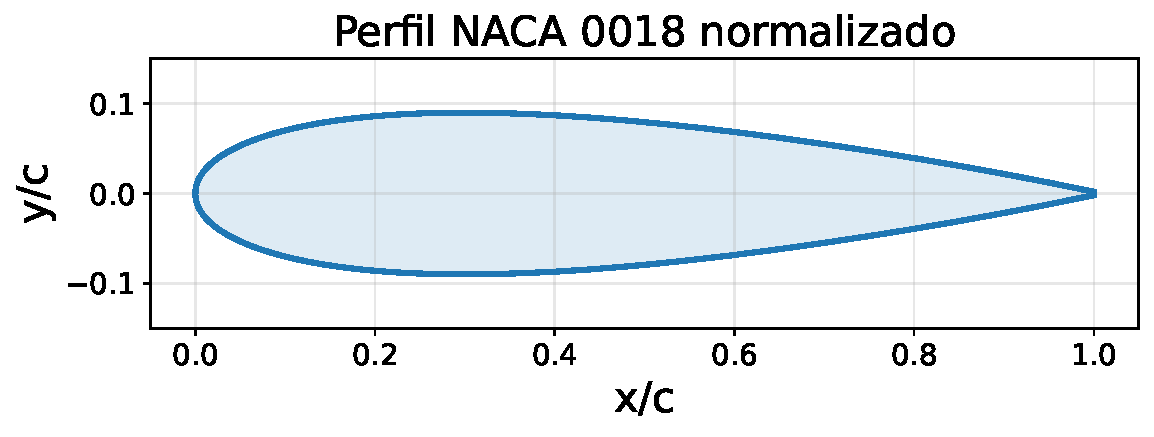
\includegraphics[width=0.7\textwidth, trim=0 0 0 25pt, clip]{Figuras/Figuras Metodología/NACA0018.pdf}
\caption{Perfil NACA 0018 normalizado.}
\label{fig:naca0018}
\end{figure}

\begin{table}[H]
    \caption{Parámetros geométricos del rotor y la pala de la turbina.}
    \label{tab:geometria_turbina}
    \begin{tabular}{lccc}
        \hline
        \textbf{Parámetro Geométrico} & \textbf{Símbolo} & \textbf{Valor} & \textbf{Unidad}\\
        \hline
        Diámetro del rotor                  & $D$     & 20{,}73 & m \\
        Radio del rotor                     & $R$     & 10{,}365 & m \\
        Largo de la pala (Altura del rotor) & $H$     & 23 & m \\
        Longitud de la cuerda de la pala    & $c$     & 1{,}1 & m \\
        Perfil alar                         & —       & NACA 0018   & — \\
        Espesor máximo del perfil           & $t$     & 0{,}198 & m \\
        Número de palas                     & $N$     & 3 & — \\
        Área de barrido del rotor           & $A_s$   & 476{,}79 & m$^2$ \\
        Posición de conexión de struts      & —       & 5{,}0 y 17{,}0 & m \\
        Masa de la pala                     & $m$     & 760 & kg \\
        \hline
    \end{tabular}
\end{table}

\section{Etapa 1: caracterización del emplazamiento y recurso eólico}

\subsection{Caracterización del recurso eólico}
\label{sec:recurso_metodo}

No es posible contar con mediciones anemométricas en el sitio de instalación, ya que por motivos de confidencialidad, no se ha presentado la ubicación exacta de este. En su lugar, se adopta como caso de estudio un emplazamiento representativo de la costa sur de Chile, con coordenadas conocidas (Sección~\ref{sec:sitio_instalacion}), sobre el cual sí es posible aplicar el procedimiento normativo completo; el objetivo es validar la metodología para que pueda reproducirse directamente cuando la ubicación real esté disponible. La caracterización del recurso en ese emplazamiento se apoya en el explorador eólico~\parencite{ExploradorEolico2018}, herramienta desarrollada por el Departamento de Geofísica de la Universidad de Chile mediante un convenio de cooperación con el Ministerio de Energía y el apoyo de la Cooperación Alemana (GIZ) para la evaluación del potencial eólico en el territorio nacional. La serie empleada corresponde a una reconstrucción climatológica de resolución horaria que abarca el periodo entre los años 1980 y 2017. La sección 11.3 de la norma IEC 61400-1~\parencite{IEC61400-1} no fija un número mínimo de años para esta caracterización, sino un mínimo de seis meses de registro, exigiendo además que el periodo sea lo bastante largo para cubrir de forma conservadora las variaciones estacionales; los 37 años de la serie satisfacen ambos requisitos con holgura. La metodología con que el explorador eólico genera y valida estas series se documenta en~\parencite{ExploradorEolico2018,Skamarock2008,Powers2017,Gelaro2017}.

\subsubsection{Caracterización analítica de la velocidad media}

La norma IEC 61400-1~\parencite{IEC61400-1} define la velocidad media anual ($V_{ave}$) como el valor esperado medido sobre una duración suficiente para promediar efectos no estacionarios. Su determinación sigue las etapas siguientes:

\begin{enumerate}
    \renewcommand{\labelenumi}{\alph{enumi})}
    \item \textbf{Ajuste por cizalladura vertical:} Se extrae la serie horaria de la reconstrucción climatológica en el nivel de extracción original ($z = 5{,}5$ m) y se extrapola a la altura del centro del rotor ($z = 21{,}3$ m) aplicando el perfil de viento normal (\gls{nwp}) descrito en la Sección~\ref{sec:condiciones_diseno} mediante la Ec.~\ref{eq:nwp_ley_potencia}, con el exponente de cizalladura $\alpha_z = 0{,}12$ adoptado para el emplazamiento offshore.

    \item \textbf{Cálculo de la media aritmética:} Sobre la serie ya extrapolada a la altura del centro del rotor, se calcula la media mediante la Ec.~\ref{eq:media_aritmetica}:
    \begin{equation}
        V_{ave} = \frac{1}{N} \sum_{i=1}^{N} V_i
        \label{eq:media_aritmetica}
    \end{equation}
    donde $V_i$ es cada uno de los $N$ registros horarios de velocidad de la serie extrapolada.

    \item \textbf{Velocidad de referencia:} A partir de la velocidad media anual ya extrapolada a la altura del centro del rotor ($V_{ave}$ a $z = 21{,}3$ m), se determina la velocidad de referencia ($V_{ref}$) definida en la Sección 6.3.1.1 de la norma IEC 61400-1~\parencite{IEC61400-1} para la clasificación de emplazamientos, según la Ec.~\ref{eq:vave_vref}:
    \begin{equation}
        V_{ave} = 0{,}2 \, V_{ref}
        \label{eq:vave_vref}
    \end{equation}

    \item \textbf{Modelado de la distribución de probabilidad:} Sobre la serie ya extrapolada a la altura del centro del rotor, la distribución de probabilidad de frecuencias ($f_W$) de la velocidad del viento se modela mediante la distribución de Weibull descrita en la Sección~\ref{sec:distribucion_viento}, cuyo ajuste permite describir la permanencia del viento en el emplazamiento. Al tratarse de una evaluación sitio-específica sobre un registro histórico, y no de la adopción de una clase estándar, ambos parámetros se ajustan por máxima verosimilitud~\parencite{Seguro2000}, en lugar de fijar $k = 2$ como en el modelo de Rayleigh de referencia. La función de densidad de probabilidad se expresa según la Ec.~\ref{eq:weibull_pdf_general}:
    \begin{equation}
        f_W(V; k, c) = \frac{k}{c} \left( \frac{V}{c} \right)^{k-1} \exp\left[ -\left( \frac{V}{c} \right)^k \right]
    \label{eq:weibull_pdf_general}
    \end{equation}
    donde $k$ es el parámetro de forma (adimensional) y $c$ el parámetro de escala (m/s), ambos determinados a la altura del centro del rotor. La estimación por máxima verosimilitud sobre los $N$ registros $V_i$ de la serie resuelve primero el parámetro de forma como raíz de la Ec.~\ref{eq:weibull_mle_k}, que no admite solución explícita y se obtiene por iteración numérica:
    \begin{equation}
        \frac{\sum_{i=1}^{N} V_i^{\,k} \ln V_i}{\sum_{i=1}^{N} V_i^{\,k}} - \frac{1}{k} - \frac{1}{N} \sum_{i=1}^{N} \ln V_i = 0
        \label{eq:weibull_mle_k}
    \end{equation}
    y a partir de ese valor obtiene el parámetro de escala por sustitución directa, según la Ec.~\ref{eq:weibull_mle_c}:
    \begin{equation}
        c = \left( \frac{1}{N} \sum_{i=1}^{N} V_i^{\,k} \right)^{1/k}
        \label{eq:weibull_mle_c}
    \end{equation}
\end{enumerate}

\subsubsection{Caracterización de la turbulencia según IEC 61400-3}
\label{sec:ntm}

Para caracterizar la turbulencia del flujo incidente se aplica el modelo de turbulencia normal (NTM) que la norma IEC 61400-3~\parencite{IEC61400-3} adopta para emplazamientos offshore, y cuya formulación se recoge en la Ec.~\ref{eq:ntm_sigma} de la Sección~\ref{sec:condiciones_diseno}. Esa expresión queda definida por dos parámetros, la intensidad de turbulencia de referencia $I_{ref}$ y el parámetro de ordenada $b_{NTM}$, que la norma tabula según la categoría de turbulencia asignada al emplazamiento~\parencite{IEC61400-1}.

La Sección 12.3 de IEC 61400-3~\parencite{IEC61400-3} establece que, a falta de datos de turbulencia del emplazamiento, la desviación estándar de la velocidad puede estimarse a partir de la rugosidad de la superficie del mar. Esa rugosidad no es un valor fijo, sino que crece con la velocidad del viento, porque es el propio viento el que levanta el oleaje que la produce. La norma recoge ese acoplamiento mediante la relación de \textcite{Charnock1955}, que vincula la longitud de rugosidad con la velocidad de fricción del flujo, según la Ec.~\ref{eq:charnock_z0}:

\begin{equation}
    z_0 = \frac{A_C}{g} \left[ \frac{\kappa \, V_{hub}}{\ln \left( z_{hub} / z_0 \right)} \right]^2
    \label{eq:charnock_z0}
\end{equation}

donde $z_0$ es la longitud de rugosidad de la superficie del mar (medida en metros), $g$ la aceleración de gravedad, la constante de von Kármán $\kappa = 0{,}4$ y la constante de Charnock $A_C$, que la norma fija en $0{,}011$ para mar abierto~\parencite{IEC61400-3}. La expresión es implícita, ya que $z_0$ aparece en ambos miembros, y se resuelve por iteración numérica. Con la rugosidad así obtenida, la desviación estándar representativa se calcula según la Ec.~\ref{eq:charnock_sigma}:

\begin{equation}
    \sigma_{NTM} = \frac{V_{hub}}{\ln \left( z_{hub} / z_0 \right)} + 1{,}28 \cdot 1{,}44 \cdot I_{ref}
    \label{eq:charnock_sigma}
\end{equation}

donde $I_{ref}$ interviene evaluado a $V_{hub} = 15$~m/s, ya que la norma lo define precisamente como el valor esperado de la intensidad de turbulencia a esa velocidad~\parencite{IEC61400-1}. Conviene precisar que esta velocidad de $15$~m/s es un punto fijo de la norma IEC 61400-1.

\subsubsection{Generación del campo de viento turbulento}
\label{sec:campo_turbulento}

Para la simulación aerodinámica en QBlade, el campo de viento incidente se genera mediante el modelo de Mann descrito en la Sección~\ref{sec:modelo_mann}, con los parámetros de turbulencia de la categoría asignada al emplazamiento (Sección~\ref{sec:ntm}). El modelo no sintetiza el viento sobre la turbina, sino sobre un volumen de aire que después se hace pasar por ella. Ese volumen es la caja de turbulencia: un prisma de velocidades fluctuantes almacenadas sobre una grilla regular de puntos, con dos direcciones transversales al flujo, que deben cubrir el plano barrido por el rotor. La Figura~\ref{fig:caja_turbulencia} ilustra la caja sintetizada para una de las realizaciones simuladas, con la turbina superpuesta a escala para dimensionar el volumen de aire generado frente al rotor.

\begin{figure}[H]
    \centering
    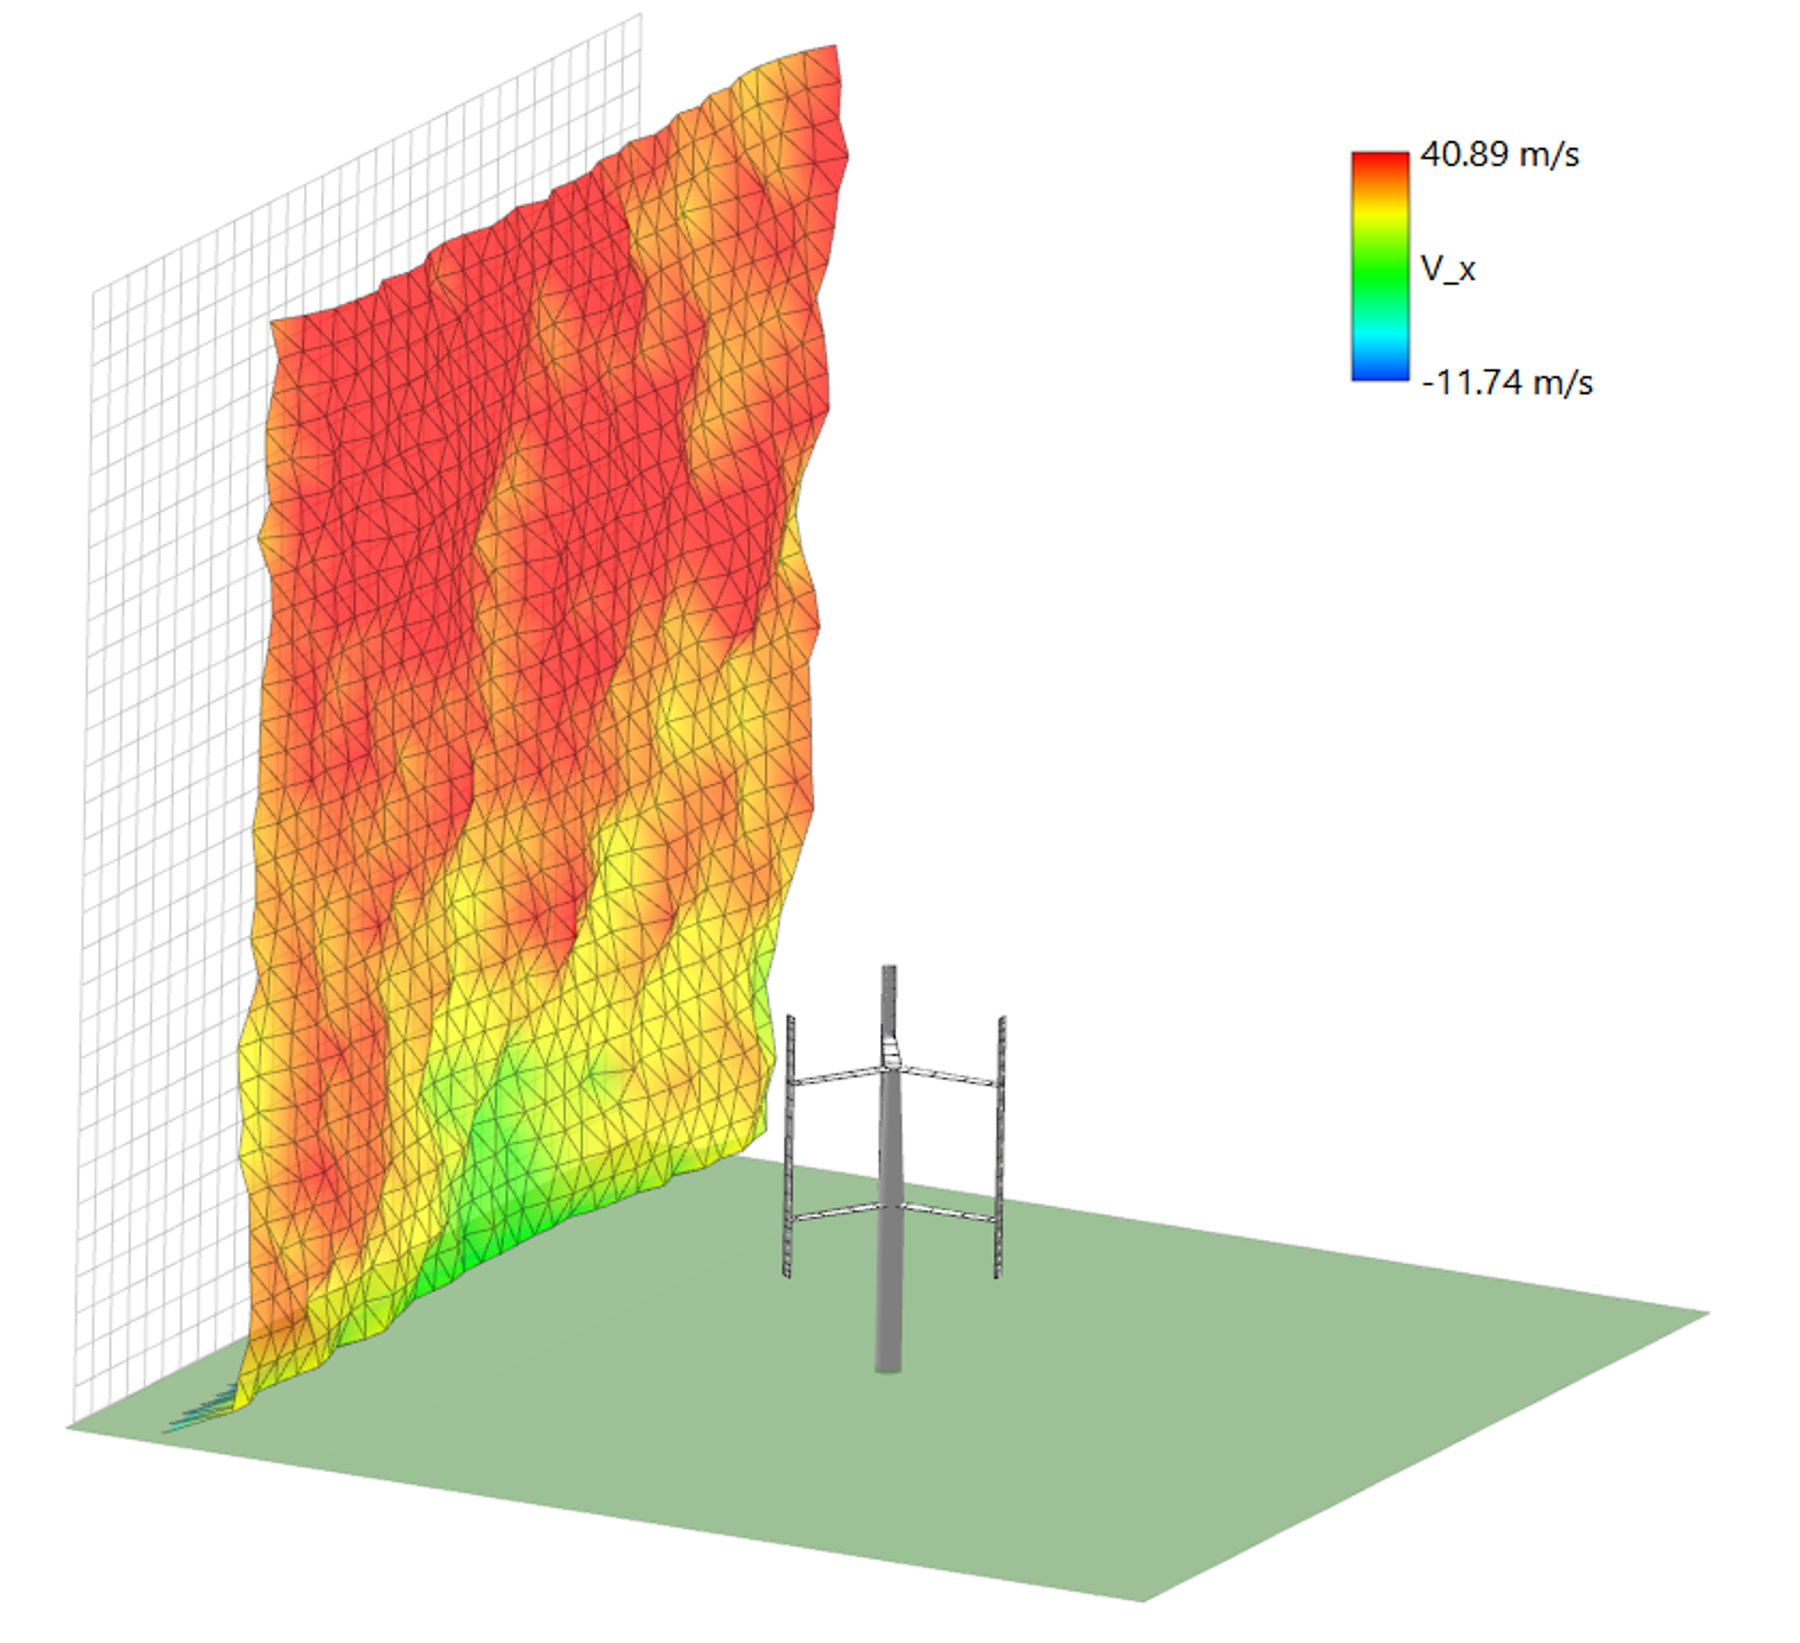
\includegraphics[width=0.7\textwidth]{Figuras/caja_turbulencia_3d.png}
    \caption[Caja de turbulencia generada por el modelo de Mann.]{Caja de turbulencia sintetizada por el modelo de Mann para una de las realizaciones simuladas, coloreada según la componente longitudinal de la velocidad ($V_x$), con la turbina superpuesta a escala.}
    \label{fig:caja_turbulencia}
\end{figure}

La sección transversal se dimensiona en $100 \times 100$~m, discretizada en $32 \times 32$ puntos, configuración empleada por Marten en sus estudios de validación del software~\parencite{marten2019qblade}. La longitud no se fija de forma independiente, ya que resulta del producto de la velocidad media del caso por la duración de la simulación.

Las dimensiones adoptadas satisfacen los requisitos aplicables de IEC 61400-1~\parencite{IEC61400-1} en dos aspectos. Por una parte, la sección transversal cubre íntegramente el plano barrido por el rotor, de $D = 20{,}73$~m de ancho y $H = 23$~m de extensión vertical: ese plano ocupa $476{,}79$~m$^2$ de los $10\,000$~m$^2$ de la sección de la caja, esto es, un $4{,}8\%$ de su área, con un dominio casi cinco veces más ancho que el rotor y más de cuatro veces más alto. El dominio cubre así el plano barrido con holgura, condición necesaria para el muestreo rotacional que la Sección 6.3 de la norma IEC 61400-1~\parencite{IEC61400-1} exige admitir al modelo de turbulencia, ya que la pala describe una trayectoria circular y en cada instante interroga puntos distintos de la grilla. Por otra parte, el Anexo B de la norma IEC 61400-1~\parencite{IEC61400-1} recomienda ajustar la factorización del tensor espectral del modelo de Mann cuando el dominio espacial es inferior a $8\ell$ en alguna de sus dimensiones, donde $\ell$ es la escala de longitud del modelo, definida en la Sección~\ref{sec:modelo_mann} como $\ell = 0{,}8\,\Lambda_1$, siendo $\Lambda_1 = 0{,}7\,z = 14{,}9$~m el parámetro de escala de turbulencia longitudinal para la altura del centro del rotor ($z = 21{,}3$~m $< 60$~m, Ecuación 5 de la norma IEC 61400-1~\parencite{IEC61400-1}). El umbral resultante, $8\ell \approx 95{,}4$~m, es inferior a los $100$~m de la caja empleada, por lo que no se requiere dicho ajuste.

La resolución de la grilla se contrasta con esa misma escala. El espaciamiento transversal es de $3{,}23$~m, resultado de repartir los $100$~m de ancho entre los $31$ intervalos de la grilla, y el longitudinal, igual al producto de la velocidad por el paso temporal, alcanza $2{,}4$~m en el caso más rápido. La escala $\ell$ equivale por tanto a casi cuatro veces el espaciamiento transversal y a unas cinco veces el longitudinal, de modo que un remolino del tamaño que concentra la energía del campo queda descrito por varios puntos de la grilla y no por uno solo. Las estructuras menores que el espaciamiento no se resuelven, y su energía se repone mediante la compensación de altas frecuencias que se describe más adelante.

La Figura~\ref{fig:mann_config} reproduce la ventana con que se configura cada caja en QBlade, ilustrada para la velocidad de $24$~m/s. Sus campos se agrupan en cuatro bloques, que se describen a continuación. Los valores numéricos de la caracterización del emplazamiento que alimentan esta ventana se reportan en el Capítulo~4.

\begin{figure}[H]
    \centering
    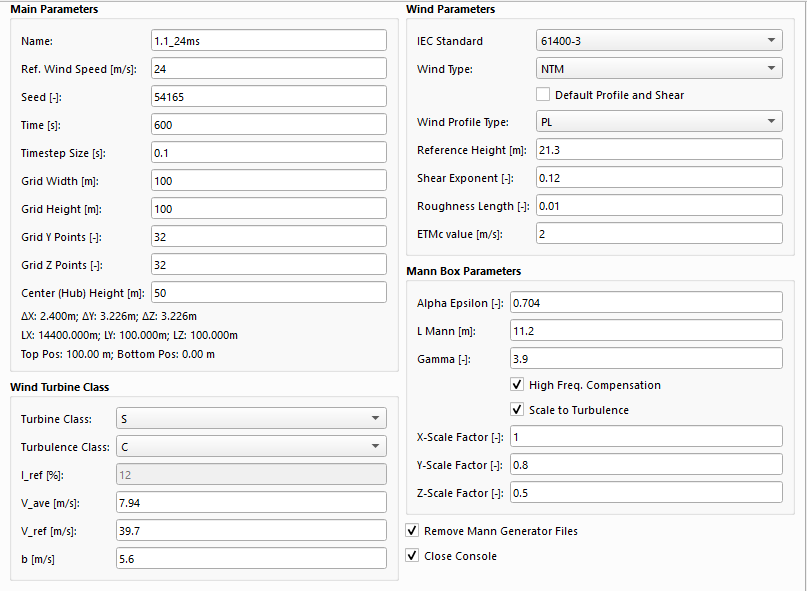
\includegraphics[width=0.7\textwidth]{Figuras/Mann.png}
    \caption[Configuración del modelo de Mann en QBlade.]{Configuración del modelo de Mann para la generación del campo de viento turbulento en QBlade, ilustrada para la velocidad de $24$~m/s.}
    \label{fig:mann_config}
\end{figure}

\textbf{Parámetros principales.} Definen la geometría de la caja y su discretización. La velocidad de referencia es la del centro del rotor del caso de carga que se simula, y la semilla es el entero que inicializa el generador de números aleatorios, distinto en cada una de las seis realizaciones de cada velocidad (Sección~\ref{sec:velocidades_simulacion}), que es lo que hace que representen realizaciones independientes del mismo proceso estocástico. La duración de $600$~s y el paso temporal de $0{,}1$~s fijan, junto con la velocidad, la longitud del dominio longitudinal y su resolución. Los campos de ancho, alto y número de puntos son los ya justificados. La altura del centro de la caja se fija en $50$~m, y no en la del centro del rotor, de modo que el dominio abarca desde el nivel del mar hasta los $100$~m, cotas que la propia ventana informa: es una posición de la caja en el espacio, no un dato de la turbina, que se declara aparte como altura de referencia.

\textbf{Clase de turbina.} La turbina se declara de clase S, denominación que la norma reserva para los emplazamientos cuyas condiciones no quedan descritas por una clase estándar~\parencite{IEC61400-1}, ya que la velocidad media y la velocidad de referencia provienen del registro del sitio (Sección~\ref{sec:recurso_metodo}) y no de los valores tabulados. La turbulencia, en cambio, se declara en la categoría asignada en la Sección~\ref{sec:ntm}, con lo que el programa toma para ella los valores que la norma tabula. Los cuatro campos que siguen recogen esa combinación: la velocidad media y la velocidad de referencia obtenidas de la caracterización del recurso, y la intensidad de turbulencia de referencia y el parámetro de ordenada propios de la categoría adoptada.

\textbf{Parámetros de viento.} Fijan el marco normativo y el perfil medio sobre el que se superpone la turbulencia. Se selecciona la norma IEC 61400-3~\parencite{IEC61400-3} por tratarse de un emplazamiento marino, y el tipo de viento es el modelo de turbulencia normal para los DLC 1.1 y 1.2; el DLC 1.3 emplea en su lugar el modelo de turbulencia extrema, cuya constante $c_{ETM} = 2$~m/s, fijada en la Sección 6.3.2.3 de la norma IEC 61400-1~\parencite{IEC61400-1}, es la que recoge el campo correspondiente. La casilla de perfil y cizalladura por defecto se deja sin marcar precisamente para introducir los valores del emplazamiento en lugar de los tabulados: el perfil se declara como ley de potencia, que es la forma que la norma da al perfil de viento normal (Sección~\ref{sec:condiciones_diseno}), con la altura de referencia del centro del rotor y el exponente de cizalladura adoptado para el sitio, los mismos con que se extrapoló la serie de viento. La longitud de rugosidad es el parámetro que gobierna el perfil logarítmico, la alternativa al de ley de potencia adoptado aquí.

\textbf{Parámetros de la caja de Mann.} Corresponden a los tres del tensor espectral descritos en la Sección~\ref{sec:modelo_mann}: el parámetro de intensidad, bajo la denominación \textit{Alpha Epsilon}, que se obtiene de la desviación estándar representativa mediante $\sigma_{iso} = 0{,}55\,\sigma_{NTM}$ y que por ello cambia con cada velocidad simulada; la escala de longitud $\ell$, bajo la denominación \textit{L Mann}; y el parámetro de anisotropía \textit{Gamma}, que la norma fija en $3{,}9$. Los factores de escala en las tres direcciones, $1$, $0{,}8$ y $0{,}5$, reproducen las razones entre las desviaciones estándar de las tres componentes de la velocidad que la norma tabula en su Anexo B, $\sigma_2 = 0{,}8\,\sigma_1$ y $\sigma_3 = 0{,}5\,\sigma_1$. Las dos casillas activadas actúan sobre la energía del campo generado. Como la síntesis se resuelve por transformada de Fourier sobre los números de onda que la grilla contiene, según se detalla en el mismo Anexo B, los mayores que su resolución quedan fuera del campo: a reponer esa fracción de energía apunta la compensación de altas frecuencias. El escalado a la turbulencia, por su parte, ajusta el campo sintetizado para que su desviación estándar coincida con la prescrita. Las dos casillas restantes gobiernan el manejo de los archivos temporales del generador y no tienen efecto sobre el campo.

\subsection{Determinación de las propiedades termofísicas del aire}
\label{sec:propiedades_aire}

La norma IEC 61400-1~\parencite{IEC61400-1} incluye la temperatura y la densidad del aire entre las condiciones ambientales que deben evaluarse para el emplazamiento (Secciones 6.4 y 11.1), y el método aerodinámico las requiere de forma explícita: la densidad escala las fuerzas que actúan sobre la pala, y la viscosidad cinemática fija el número de Reynolds con el que se interpolan las polares del perfil durante la simulación~\parencite{marten2019qblade}. Ese número de Reynolds condiciona el resultado aerodinámico, porque las polares varían con él de forma apreciable dentro del rango en que opera la turbina, según se expone en la Sección~\ref{sec:polares}. Adoptar las propiedades de la atmósfera estándar, definidas a $15$~\textdegree C~\parencite{Anderson2016}, desplazaría por tanto el rango de Reynolds del cálculo respecto del que la pala experimenta en un emplazamiento cuya temperatura media difiere de ese valor. Por esta razón las propiedades se determinan a partir de la climatología mensual del sitio (Capítulo~4) mediante las correlaciones analíticas de uso establecido en la literatura aerodinámica para evaluar las propiedades de transporte de un gas en función de su temperatura~\parencite{White2006,Anderson2016}, en lugar de tomarse de una tabla a temperatura fija.

La viscosidad dinámica se calcula mediante la ley de Sutherland~\parencite{Sutherland1893}, correlación de referencia para la dependencia de la viscosidad de un gas con la temperatura y de uso estándar para el aire~\parencite{White2006}, según la Ec.~\ref{eq:sutherland}:

\begin{equation}
    \mu = \mu_0 \frac{T_0 + C}{T + C} \left( \frac{T}{T_0} \right)^{3/2}
    \label{eq:sutherland}
\end{equation}

donde $T$ es la temperatura del aire, $\mu_0 = 1{,}7894 \times 10^{-5}$ kg/(m·s) y $T_0 = 288{,}16$ K son la viscosidad y la temperatura del aire en las condiciones de la atmósfera estándar a nivel del mar~\parencite{Anderson2016}, par que constituye el punto de referencia de la correlación, y $C = 110{,}4$ K es la constante de Sutherland para el aire~\parencite{White2006}.

La densidad del aire se calcula mediante la ecuación de estado de los gases ideales~\parencite{Anderson2016}, aplicable al aire en el rango de presiones y temperaturas del emplazamiento, con $P_{atm} = 101325$ Pa ($1$ atm), valor de la presión atmosférica a nivel del mar según la atmósfera estándar~\parencite{Anderson2016}, de acuerdo con la Ec.~\ref{eq:densidad_aire}:

\begin{equation}
    \rho = \frac{P_{atm}}{R_a \cdot T}
    \label{eq:densidad_aire}
\end{equation}

donde $R_a = 287{,}05$ J/(kg·K) es la constante del gas para el aire seco~\parencite{Anderson2016}.

Ambas propiedades se combinan en la viscosidad cinemática, magnitud que interviene en el número de Reynolds y que se define como el cociente entre la viscosidad dinámica y la densidad~\parencite{White2006}, según la Ec.~\ref{eq:visc_cinematica}:

\begin{equation}
    \nu = \frac{\mu}{\rho}
    \label{eq:visc_cinematica}
\end{equation}

donde $\mu$ es la viscosidad dinámica obtenida de la Ec.~\ref{eq:sutherland} y $\rho$ la densidad de la Ec.~\ref{eq:densidad_aire}, ambas evaluadas a la temperatura media del emplazamiento. El valor resultante se presenta en el Capítulo~4.


\section{Etapa 2: modelado aerodinámico}

De las familias de métodos aerodinámicos comparadas en la Tabla~\ref{tab:comparacion_metodos}, se adopta el método de línea sustentadora con estela de vórtice libre (\gls{llfvw}), implementado en el software QBlade~\parencite{marten2019qblade}. El criterio de selección responde a las exigencias de la verificación normativa: los casos de carga requieren $72$ realizaciones de varios minutos con acoplamiento aeroelástico, volumen incompatible con el costo del CFD, mientras que el carácter inestable del flujo en un H-rotor y la interacción de la pala con su propia estela quedan fuera del alcance del DMST. El modelo DMST se reserva, por su bajo costo, para la estimación preliminar del \gls{tsr} óptimo (Sección~\ref{sec:dmst}), que sirve de punto de partida para las simulaciones LLFVW.

Tanto QBlade como el método empleado se apoyan en polares que describen las cargas sobre el perfil, y esas polares deben cubrir todo el rango de funcionamiento de la turbina. Como el fabricante no proporciona los parámetros operacionales, dicho rango se determina en los pasos que siguen.

\subsection{Determinación del rango operativo del número de Reynolds}
\label{sec:reynolds}

Debido a la cinemática de las \gls{vawt}, el perfil alar experimenta una velocidad relativa variable según su posición en la trayectoria circular, por lo que el número de Reynolds también varía durante la operación. Para determinar el intervalo operativo utilizado en el cálculo de polares, se evalúa la velocidad relativa $W$ en función del ángulo azimutal $\theta$, según la Ec.~\ref{eq:W_theta}:

\begin{equation}
    W(\theta) = V_{hub} \sqrt{1 + 2\lambda \cos\theta + \lambda^2}
    \label{eq:W_theta}
\end{equation}

donde $V_{hub}$ es la velocidad del viento a la altura del centro del rotor y $\lambda$ la relación de velocidad de punta. Los valores extremos de $W$ ocurren en las posiciones de barlovento ($\theta = 0^\circ$) y sotavento ($\theta = 180^\circ$), donde la expresión se simplifica según las Ecs.~\ref{eq:W_max} y~\ref{eq:W_min}:

\begin{equation}
    W_{max} = V_{hub} + \Omega R
    \label{eq:W_max}
\end{equation}

\begin{equation}
    W_{min} = |V_{hub} - \Omega R|
    \label{eq:W_min}
\end{equation}


La condición operacional más exigente para el perfil corresponde a la velocidad de corte $V_{out}$ con el rotor girando a su velocidad máxima, resultando una velocidad relativa máxima $W_{max}$. A partir de la cuerda del perfil y la viscosidad cinemática, el número de Reynolds se calcula según la Ec.~\ref{eq:Re_max_theoretical}:

\begin{equation}
    Re_{max} = \frac{W_{max} \cdot c}{\bar{\nu}}
    \label{eq:Re_max_theoretical}
\end{equation}

donde $\bar{\nu}$ es la viscosidad cinemática media del aire en el emplazamiento, obtenida según el procedimiento de la Sección~\ref{sec:propiedades_aire} y reportada en el Capítulo~4. Este valor constituye una referencia determinística para el régimen de producción de potencia, ya que la turbina se desconecta para $V > V_{out}$; las fluctuaciones turbulentas instantáneas pueden excederlo transitoriamente. Ese valor, redondeado al millón siguiente, define el límite superior del cálculo de polares. El rango paramétrico $\lambda \in [2{,}5; 4{,}5]$ y $V \in [2; 25]$~m/s constituye una envolvente teórica preliminar que abarca todas las combinaciones posibles de \gls{tsr} y velocidad de viento. El intervalo de $\lambda$ queda contenido en el documentado para las configuraciones H-Darrieus (Tabla~\ref{tab:tabla_vawt}), y el de velocidades corresponde al rango operacional adoptado en la Sección~\ref{sec:control}. El número de Reynolds operacional, verificado mediante las simulaciones \gls{llfvw}, se presenta en el Capítulo~4.

Una vez definido el rango de Reynolds, se procede al cálculo de las curvas polares mediante la siguiente estrategia de discretización, resumida en la Tabla~\ref{tab:reynolds_discretizacion}.

\begin{table}[H]
    \centering
    \caption{Estrategia de discretización del número de Reynolds para el cálculo de polares.}
    \label{tab:reynolds_discretizacion}
    \begin{tabular}{lcc}
        \hline
        \textbf{Rango} & $\Delta Re$ & \textbf{Fuente} \\
        \hline
        $60$k -- $300$k & --- & \cite{Bianchini2015} \\
        $350$k -- $1$M & $50\,000$ & QFoil \\
        $1$M -- $3$M   & $125\,000$ & QFoil \\
        $3$M -- $6$M   & $250\,000$ & QFoil \\
        \hline
    \end{tabular}
\end{table}

El cálculo con QFoil se inicia en $Re = 3{,}5 \times 10^5$, ya que por debajo de $Re = 2{,}5 \times 10^5$ no se alcanza la convergencia numérica del solucionador. Se decide cubrir el rango inferior con las polares experimentales de \textcite{Bianchini2015} para el perfil NACA 0018 ($Re = 0{,}6$; $1{,}5$; $2{,}5$ y $3{,}0 \times 10^5$), digitalizadas de las mediciones en túnel de viento publicadas e ingresadas a QBlade como tablas de puntos de $C_l$ y $C_d$ frente al ángulo de ataque, en el mismo formato con que el programa recibe las calculadas. Recurrir a esa fuente mantiene la coherencia del conjunto, porque es la misma contra la que se resuelven el criterio de transición (Sección~\ref{sec:calculo_polares}) y los parámetros del modelo de extrapolación (Sección~\ref{sec:extrapolacion_polares}): las polares de bajo Reynolds no son un dato ajeno añadido al margen, sino el patrón de contraste con el que se calibra el resto del conjunto.


\subsection{Cálculo de polares}
\label{sec:calculo_polares}

Se calculan las curvas polares mediante QFoil, preferible a XFoil en el régimen de pérdida profunda propio de una \gls{vawt} por las razones expuestas en la Sección~\ref{sec:polares}. Se utilizan los siguientes parámetros de configuración:

\begin{itemize}
    \item \textbf{Número de Mach:} La velocidad relativa máxima del rotor (Sección~\ref{sec:reynolds}), contrastada con la velocidad del sonido evaluada a la temperatura mínima del emplazamiento, arroja un número de Mach máximo del orden de $0{,}2$, muy por debajo del umbral de $0{,}3$ bajo el cual la variación de densidad sobre el perfil es despreciable (Sección~\ref{sec:polares}). El flujo admite por tanto tratarse como incompresible en todo el rango operacional, y el valor de Mach se fija en $0$ para que el solucionador prescinda de la corrección de compresibilidad de Kármán-Tsien~\parencite{Karman1941,Tsien1939}, cuya aplicación no aportaría precisión y sí introduciría una fuente adicional de error en el cálculo de las polares.

    \item \textbf{Criterio de transición ($N_{crit}$):} Las curvas polares se calculan para seis valores de $N_{crit}$: $4$, $6$, $7$, $9$, $11$ y $12$. Los valores se seleccionan a partir del valor de referencia de túnel de viento promedio ($N_{crit}=9$), explorando valores menores para representar entornos de mayor turbulencia y valores superiores para condiciones de flujo más limpio, conforme a los rangos descritos en la Tabla~\ref{tab:ncrit_values}. El valor adoptado para las simulaciones se resuelve comparando las seis polares con los datos experimentales de \textcite{Bianchini2015} a $Re = 2{,}5 \times 10^5$, y se presenta en el Capítulo~4.
    
    \item \textbf{Transición de capa límite:} Los parámetros \textit{Forced Top Transition} y \textit{Forced Bottom Transition} se fijan en $1{,}0$, permitiendo que el modelo de transición natural actúe a lo largo de toda la cuerda del perfil.

    \item \textbf{Panelado del perfil:} Se ajusta el panelado del perfil a 220 paneles con distribución de coseno~\parencite{drela1989xfoil}.
\end{itemize}

\subsection{Metodología de extrapolación de polares}
\label{sec:extrapolacion_polares}

Para simular el rendimiento del rotor de eje vertical (\gls{vawt}), se implementa el modelo de \textcite{montgomerie2004methods} en QBlade. La determinación de los parámetros del modelo se basa en los siguientes criterios:

\textbf{Determinación del coeficiente de arrastre a 90° ($C_{d90}$):} El parámetro $C_{d90}$ define la amplitud de las curvas en régimen de pérdida profunda. Su valor se determina a partir de los datos experimentales en túnel de viento de \textcite{Bianchini2015} para el perfil NACA 0018 a $Re = 2{,}5 \times 10^5$, y se reporta en el Capítulo~4.

\textbf{Determinación de la pendiente de sustentación:} La pendiente de la parte lineal de la curva de sustentación es calculada automáticamente por QBlade mediante un ajuste lineal de mínimos cuadrados de primer orden sobre el intervalo de las soluciones de QFoil comprendido entre $\alpha = -5^\circ$ y $\alpha = 5^\circ$~\parencite{marten2019qblade}.

\textbf{Configuración de los parámetros de acoplamiento ($A$ y $B$):} Estos coeficientes adimensionales controlan la forma y la suavidad de la curva extrapolada en los rangos de transición hacia el comportamiento de placa plana. Para perfiles simétricos, los valores positivos y negativos se configuran con idéntico valor absoluto ($A+ = A-$ y $B+ = B-$) para mantener la consistencia física. Su ajuste se realiza de manera visual en QBlade, tomando como referencia los datos experimentales de \textcite{Bianchini2015}, con el criterio de lograr una transición asintótica y libre de discontinuidades inmediatamente después del punto de pérdida original de QFoil.

\subsection{Estimación preliminar del TSR óptimo mediante DMST}
\label{sec:dmst}

Como paso previo a las simulaciones de alta fidelidad con \gls{llfvw}, se emplea el \gls{dmst}, descrito en la Sección~\ref{sec:metodos_aerodinamicos}, para obtener una primera estimación del \gls{tsr} óptimo de la turbina. La simulación se configura con el modelo de pérdida de punta activado, ya que, el \gls{dmst}, al representar el rotor mediante tubos de corriente bidimensionales independientes, el método asume implícitamente una pala de envergadura infinita y no reproduce por sí solo la pérdida de sustentación hacia la punta, producida por los vórtices que allí se desprenden~\parencite{marten2019qblade}. La pala se discretiza en $50$ elementos, y las propiedades del fluido se calculan a partir del análisis de viento y temperatura del emplazamiento. El barrido se ejecuta sobre un rango de velocidades de viento de $2$ a $25$ m/s con incrementos de $0{,}1$ m/s y velocidad de rotación $\Omega$ de $3$ a $42$ rpm con incrementos de $0{,}1$ rpm. De cada combinación $(V, \Omega)$ se obtiene el \gls{tsr} como $\lambda = \Omega R / V$. El \gls{tsr} correspondiente al máximo $C_p$ de cada curva proporciona el valor de referencia para configurar las simulaciones aerodinámicas posteriores.

\subsection{Definición de la turbina en QBlade}

\subsubsection{Discretización e instrumentación de la pala}
\label{sec:discretizacion}

La definición de la turbina en QBlade requiere establecer dos esquemas de discretización independientes para la pala: uno aerodinámico, que gobierna la resolución del método de vórtices libres, y uno que fija las estaciones donde se instrumenta la pala para extraer las fuerzas aerodinámicas.

\textbf{Panelado aerodinámico:} Para la resolución del método \gls{llfvw}, la pala se divide en 21 paneles con distribución de tipo coseno, que reduce el tamaño de los paneles hacia la punta de la pala para capturar mejor los mayores gradientes de circulación que ahí se presentan, configuración con la que \textcite{marten2019qblade} valida el método en QBlade; la documentación del software describe las configuraciones alternativas disponibles~\parencite{QBladeDocs2024}. Entre paneles contiguos, la circulación se interpola mediante splines cúbicos de clase C2, polinomios que empalman sin discontinuidades hasta su segunda derivada. La Figura~\ref{fig:panelado_aerodinamico} muestra la distribución resultante sobre las tres palas del rotor.

\begin{figure}[H]
\centering
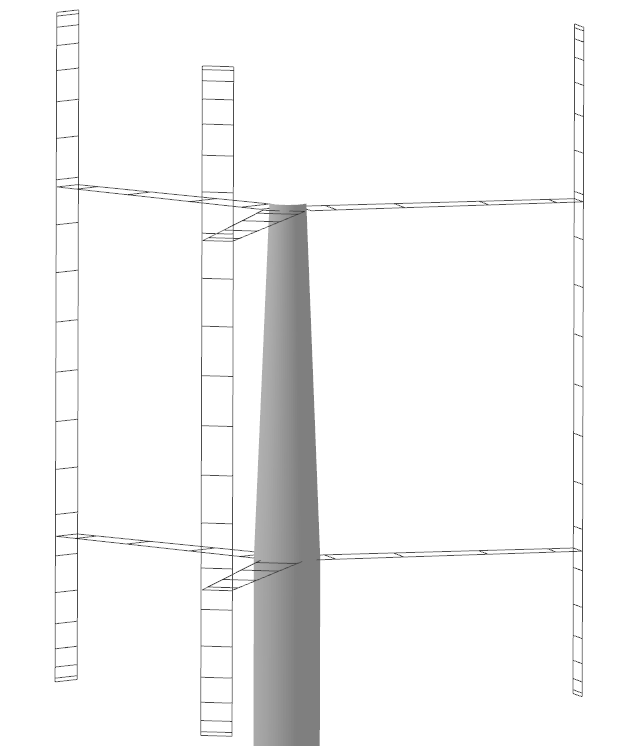
\includegraphics[width=0.55\textwidth]{Figuras/Figuras Metodología/panelado_aerodinamico.png}
\caption[Panelado aerodinámico del rotor en QBlade.]{Panelado aerodinámico de las tres palas del rotor en QBlade, según la distribución de tipo coseno descrita en el texto.}
\label{fig:panelado_aerodinamico}
\end{figure}

\textbf{Estaciones de extracción de cargas:} La pala se discretiza en 23 elementos uniformemente espaciados ($\Delta = 0{,}0435$), definiendo 24 estaciones desde la raíz ($s = 0$) hasta la punta ($s = 1$), separadas aproximadamente $1$~m entre sí, criterio con que se resolvió instrumentar la pala. En cada una de esas estaciones se dispone un sensor, lo que con tres palas resulta en 72 puntos de medición. Cada sensor registra las fuerzas aerodinámicas en los tres ejes del sistema local de la pala, cuyas direcciones se definen en la Figura~\ref{fig:ejes_locales}, las coordenadas y velocidades en el sistema de referencia global, las aceleraciones lineales y angulares, y los datos aerodinámicos correspondientes a cada estación (ángulo de ataque local, velocidades relativas y coeficientes aerodinámicos). De esta configuración se obtienen las series temporales completas de fuerzas incidentes a lo largo de la envergadura, que constituyen la entrada directa del análisis por elementos finitos de la pala (Sección~\ref{sec:fem}).

\begin{figure}[H]
\centering
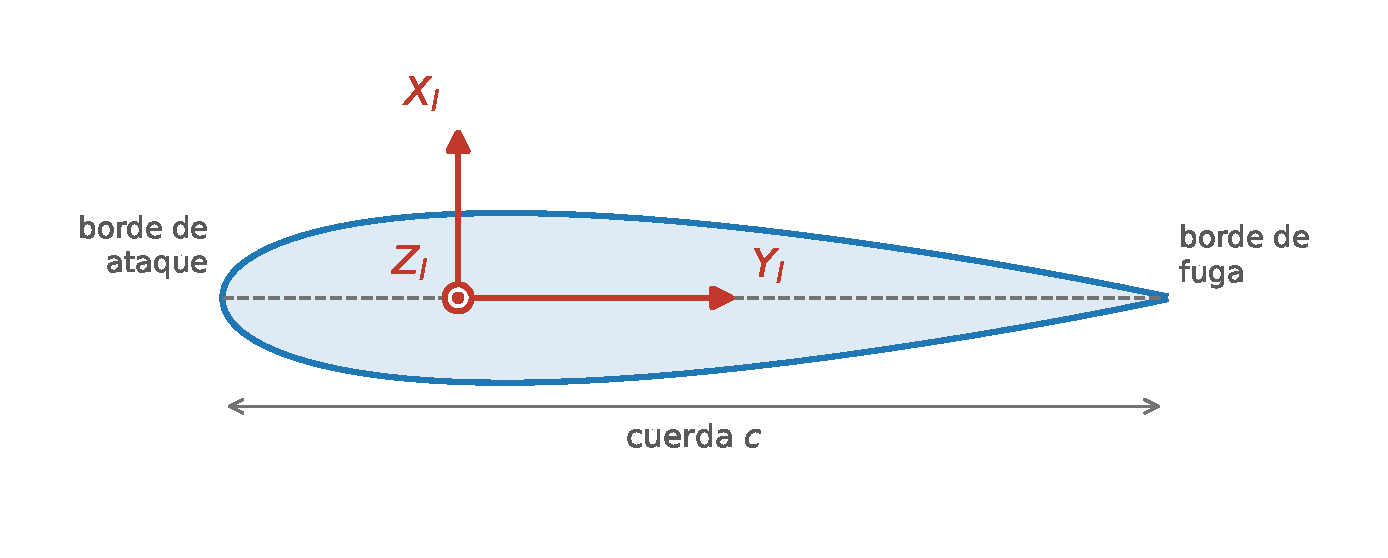
\includegraphics[width=0.75\textwidth]{Figuras/Figuras Metodología/ejes_locales_pala.pdf}
\caption[Sistema de ejes locales de la pala.]{Sistema de ejes locales de la pala sobre la sección del perfil: $X_l$ normal a la cuerda, $Y_l$ en el sentido de la cuerda hacia el borde de fuga y $Z_l$ a lo largo de la envergadura hacia la punta.}
\label{fig:ejes_locales}
\end{figure}

\subsubsection{Modelos aerodinámicos y pérdida dinámica}

Para la simulación en QBlade se selecciona el modelo de pérdida dinámica Gormont-Berg con constante de corrección $A_m = 6$, valor con el que \textcite{marten2019qblade} valida el modelo sobre un rotor Darrieus.

Los submodelos aerodinámicos complementarios que ofrece el software se configuran según su aplicabilidad a la geometría del rotor y a los grados de libertad del modelo. La aerodinámica no circulatoria, que incorpora el término de masa añadida asociado a la tasa de cabeceo por deformación torsional y a la deflexión de un flap~\parencite{marten2019qblade}, se mantiene desactivada, ya que el modelo no contempla flaps ni grado de libertad torsional. La corrección de sustentación y arrastre en dos puntos, se desactiva por corresponder a geometrías de diedro o cono, que las palas de un H-rotor de palas rectas no presenta~\parencite{QBladeDocsAero2024}. El efecto Himmelskamp, que describe el retraso de la pérdida producido por el adelgazamiento centrífugo de la capa límite y por la fuerza de Coriolis sobre una pala en rotación, y que QBlade implementa mediante la corrección de Snel~\parencite{marten2019qblade}, queda igualmente desactivado: dicha corrección escala con la razón entre la cuerda y la posición radial del elemento, magnitud que no varía en una pala que recorre su envergadura a radio constante. Se activa, en cambio, el modelo de sombra de torre, que superpone la solución de flujo potencial alrededor de un cilindro con un modelo de estela gobernado por el coeficiente de arrastre de la torre~\parencite{marten2019qblade}, ya que la pala describe su trayectoria en torno al eje central de la turbina y este perturba el flujo incidente. No se dispone del diámetro de ese eje, dato que fijaría el número de Reynolds del flujo a su alrededor y con él el valor preciso del coeficiente de arrastre. Ante esa indeterminación se adopta $C_{d,torre} = 1{,}0$, coherente con los valores que se manejan para secciones circulares en flujo transversal~\parencite{White2006}. Esta configuración se muestra en la Figura~\ref{fig:qblade_dynamic_stall}, tomada del módulo de definición de la turbina. Además de ser el valor utilizado por~\textcite{marten2019qblade}.

\begin{figure}[H]
\centering
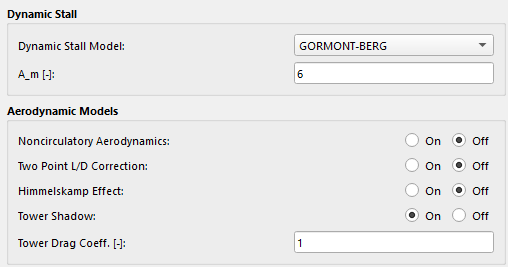
\includegraphics[width=0.6\textwidth]{Figuras/Figuras Metodología/qblade_dynamic_stall.png}
\caption{Modelo de pérdida dinámica Gormont-Berg y submodelos aerodinámicos configurados en el módulo de definición de la turbina de QBlade.}
\label{fig:qblade_dynamic_stall}
\end{figure}

\subsubsection{Modelo de estela LLFVW}

Para la resolución de la inducción del rotor se utiliza el método \gls{llfvw}. El esquema de integración de la convección de la estela se fija en Predictor-Corrector Backwards (PC2B), de segundo orden. Frente al esquema de primer orden de Euler, este duplica el número de evaluaciones del campo de velocidades por paso temporal, pero la mayor precisión que alcanza permite emplear un paso mayor manteniendo una exactitud aceptable~\parencite{marten2019qblade}, compensación pertinente en un conjunto de $102$ simulaciones de $600$~s.

Se habilita la auto-inducción de la estela (\textit{Wake Rollup}), sin la cual los filamentos no se deforman bajo su propio campo inducido y la estela deja de ser libre, condición que el método requiere para resolver la interacción de la pala con su propia estela. Se incluyen tanto los vórtices de arrastre (\textit{trailing}), que recogen la variación de la circulación ligada a lo largo de la envergadura, como los de desprendimiento (\textit{shed}), que recogen su variación en el tiempo. \textcite{marten2019qblade} señala que la circulación de estos últimos tiende a cero en simulaciones estacionarias con flujo incidente constante, caso en que su omisión acelera el cálculo sin pérdida apreciable. Esa condición no se cumple aquí, ya que el flujo incidente es turbulento y la circulación ligada varía además con el acimut a lo largo de cada revolución.

El transporte de los nodos de la estela (\textit{Wake Convection}) se configura en modo local, en el que la velocidad de convección se evalúa en la posición de cada nodo, en lugar de emplear la velocidad constante a la altura del centro del rotor o el perfil medio de la capa límite~\parencite{QBladeDocsAero2024}. Esta opción es la consistente con un campo de viento turbulento generado mediante el modelo de Mann, cuyas fluctuaciones varían en el espacio y en el tiempo.

La resolución del método LLFVW requiere definir los parámetros que controlan la discretización de la estela y el modelado de los vórtices, los cuales determinan la estabilidad numérica y la resolución espacial de la simulación. Estos parámetros se resumen en la Tabla~\ref{tab:parametros_estela}.

\begin{table}[H]
    \centering
    \caption{Parámetros de la estela y del modelado de vórtices configurados en QBlade.}
    \label{tab:parametros_estela}
    \begin{tabular}{lcc}
        \hline
        \textbf{Parámetro} & \textbf{Valor} & \textbf{Unidad} \\
        \hline
        \multicolumn{3}{c}{\textit{Malla de vórtices}} \\
        \hline
        Wake Relaxation Factor & $0{,}5$ & — \\
        Máximo de elementos de estela & $2 \times 10^5$ & — \\
        Distancia de truncamiento & $30$ & radios de rotor \\
        Wake Reduction Factor & $0{,}004$ & — \\
        Wake Zones (N/1/2/3) & $1$ / $4$ / $8$ / $12$ & revoluciones del rotor \\
        Refinamiento Streamwise (1/2/3) & $2$ / $2$ / $2$ & revoluciones del rotor \\
        Refinamiento Spanwise (1/2/3) & $1$ / $1$ / $2$ & revoluciones del rotor \\
        \hline
        \multicolumn{3}{c}{\textit{Modelado de vórtices}} \\
        \hline
        Bound Core Radius & $0{,}3$ & — \\
        Wake Core Radius & $0{,}1$ & — \\
        Turbulent Vortex Viscosity & $100$ & — \\
        Vortex Stretching & ON & — \\
        Max Vortex Stretching Factor & $50$ & — \\
        \hline
        \multicolumn{3}{c}{\textit{Iteración Gamma}} \\
        \hline
        Max Epsilon & $10^{-3}$ & — \\
        Max Number of Iterations & $100$ & — \\
        \hline
    \end{tabular}
\end{table}

Los valores adoptados provienen de la configuración con que \textcite{marten2019qblade} simula rotores Darrieus en QBlade, o se derivan de los criterios que esa misma fuente y la documentación del programa establecen. La longitud total de la estela, de $12$ revoluciones, es la que el autor reporta para su caso \gls{vawt} y la que, al \gls{tsr} de diseño, mantiene el error del coeficiente de potencia por debajo del $1\%$. Las zonas en que esa longitud se subdivide responden al método de engrosamiento progresivo de la estela, que reduce la resolución del reticulado por un factor entero cada vez que los filamentos alcanzan la edad que delimita cada zona; los factores en la dirección de la corriente reproducen el valor de $2$ del ejemplo documentado por el autor, mientras que en la dirección de la envergadura el engrosamiento se reserva para la última zona, la más alejada del rotor y la de menor influencia sobre la inducción. El factor de reducción adaptativa, de $0{,}004$, descarta los filamentos cuya circulación cae por debajo de esa fracción de la máxima presente en la estela~\parencite{QBladeDocsAero2024}, con lo que la misma fuente reporta una disminución del número de elementos a la mitad sin efecto apreciable sobre la exactitud; es además un valor más conservador que el que allí se emplea para \gls{vawt}, ya que descarta menos filamentos. El factor de relajación de la estela, de $0{,}5$, gobierna el desvanecimiento progresivo del vórtice de arranque, cuyo efecto sobre la solución se diluye así a medida que la estela se desarrolla~\parencite{QBladeDocsAero2024}. La distancia de truncamiento, expresada en radios de rotor, y el máximo de elementos operan como topes sobre el crecimiento del reticulado.

En el modelado de los vórtices, ambos radios de núcleo se definen como fracción de la cuerda local~\parencite{QBladeDocsAero2024}: el de la estela, de $0{,}1$, corresponde al $10\%$ que el autor propone como tamaño inicial del núcleo de los filamentos que se desprenden del borde de fuga, y el ligado, de $0{,}3$, fija el núcleo de los vórtices adheridos a la pala. La viscosidad turbulenta de $100$ es la que \textcite{marten2019qblade} reporta para su caso \gls{vawt}, y junto con los radios interviene en la ley con que el núcleo del vórtice crece a lo largo del tiempo. Activar el estiramiento de vórtices incorpora a esa misma ley la tasa de deformación del filamento, de modo que el núcleo responde al alargamiento que sufre al convectarse; el factor máximo de estiramiento, de $50$, es el umbral de deformación acumulada a partir del cual el filamento se retira de la estela~\parencite{QBladeDocsAero2024}.

La iteración Gamma, descrita en la Sección~\ref{sec:metodos_aerodinamicos}, resuelve la circulación ligada de los paneles en cada paso temporal. Sus dos parámetros acotan ese lazo: la circulación se actualiza hasta satisfacer el criterio de convergencia, fijado en $10^{-3}$, o hasta alcanzar el número máximo de iteraciones, fijado en $100$~\parencite{QBladeDocsAero2024}. El primero determina con qué exactitud queda resuelta la circulación antes de avanzar al paso siguiente; el segundo acota el costo y evita que un paso que no converja detenga la simulación.

Las Figuras~\ref{fig:qblade_wake_modeling} y~\ref{fig:qblade_vortex_modeling} muestran la configuración descrita en la interfaz de QBlade.

\begin{figure}[H]
\centering
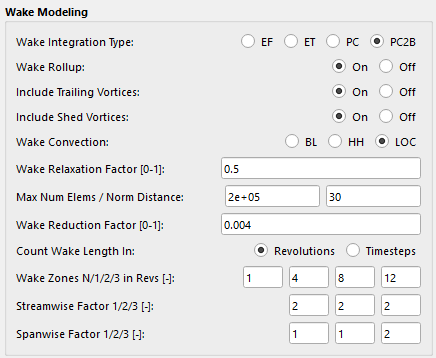
\includegraphics[width=0.5\textwidth]{Figuras/Figuras Metodología/qblade_wake_modeling.png}
\caption{Configuración de la estela, parámetros de truncamiento y refinamiento direccional en QBlade.}
\label{fig:qblade_wake_modeling}
\end{figure}

\begin{figure}[H]
\centering
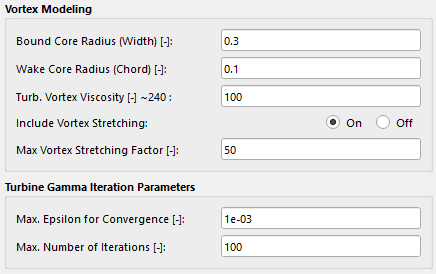
\includegraphics[width=0.5\textwidth]{Figuras/Figuras Metodología/qblade_vortex_modeling.png}
\caption{Modelado de vórtices y parámetros de convergencia de la iteración Gamma en QBlade.}
\label{fig:qblade_vortex_modeling}
\end{figure}

\subsubsection{Discretización temporal}
\label{sec:discretizacion_temporal}

La discretización temporal se especifica como un incremento acimutal y no como un paso de tiempo fijo. Se adopta $\Delta\theta = 5^\circ$, el incremento que \textcite{marten2019qblade} recomienda para la simulación aerodinámica y emplea en sus estudios sobre rotores Darrieus.

Definir el criterio sobre el ángulo y no sobre el tiempo lo independiza de la velocidad de rotación. El paso temporal queda determinado por $\Delta t = \Delta\theta / \Omega$, evaluado con la velocidad de rotación que la estrategia de control de la Sección~\ref{sec:control} asigna a cada velocidad de viento y mantenido fijo durante la simulación. Cada caso recibe así su propio paso, el mayor en $V_{in}$, donde la rotación es más lenta, y el menor una vez que esta alcanza su límite de diseño. Todos conservan los mismos $72$ pasos por revolución aunque $\Omega$ varíe con la velocidad del viento.

\subsubsection{Estrategia de control del rotor}
\label{sec:control}

Debido a que el campo de viento incorpora turbulencia, la velocidad incidente varía a lo largo de la simulación. Se implementa por ello el sistema de control descrito en la Sección~\ref{sec:control_teoria}, que mantiene el rotor en su \gls{tsr} óptimo, de modo que las simulaciones representen el funcionamiento normal de la turbina. Esta estrategia se adopta además por una razón de implementación, ya que es la que el programa admite integrar directamente en la simulación a través de su interfaz de controladores, sin requerir el desarrollo de una biblioteca de control propia~\parencite{QBladeDocsController2024}.

El rotor opera bajo dos regímenes, separados por la velocidad de viento a la que la rotación alcanza su valor máximo de diseño. Por debajo de esa velocidad se emplea el controlador $K$-$\omega^2$ de la Ec.~\ref{eq:K_omega2}, cuya constante se evalúa mediante la Ec.~\ref{eq:K_derivation} con los parámetros de diseño del rotor ($\rho = 1{,}225$~kg/m$^3$, $A = 476{,}79$~m$^2$, $R = 10{,}365$~m, $\lambda = 3{,}80$) y un coeficiente de potencia representativo $C_p = 0{,}45$. El valor resultante se presenta en el Capítulo~4.

Por sobre ella el controlador se desactiva y la velocidad de rotación se mantiene en ese valor máximo. Esta consigna se obtiene aplicando el criterio de la Sección~\ref{sec:criterio_rotacion}, que evalúa la Ec.~\ref{eq:omega_from_vtip} con el \gls{tsr} objetivo y la velocidad de viento nominal. El \gls{tsr} proviene del barrido DMST de la Sección~\ref{sec:dmst}, ejecutado como paso previo a las simulaciones de alta fidelidad precisamente para fijarla. La velocidad de viento nominal, que el fabricante no especifica, se adopta por analogía con las máquinas H-rotor de potencia y escala comparables, que alcanzan sus $200$~kW nominales a $12$~m/s (Tabla~\ref{tab:hrotor_rpm}). El desarrollo del cálculo, su contraste con el límite documentado para la T1-turbine y la solicitación centrífuga que la consigna implica se presentan en el Capítulo~4.

Los parámetros operacionales adoptados para las simulaciones se resumen en la Tabla~\ref{tab:parametros_operacionales}. A diferencia de los parámetros geométricos y de material (Tablas~\ref{tab:geometria_turbina} y~\ref{tab:material_pala}), estos no los proporciona el fabricante, sino que se definen por criterio de diseño a partir del análisis del recurso eólico y de la turbina de referencia.

Los dos límites del rango operacional se adoptan igualmente por criterio de diseño. La velocidad de arranque se fija en $V_{in} = 2$~m/s, y su plausibilidad se verifica a posteriori mediante las simulaciones \gls{llfvw}, que confirman la operación del rotor a esa velocidad (Capítulo~4). La velocidad de corte se fija en $V_{out} = 25$~m/s, valor que coincide con el documentado para la T1-turbine (Tabla~\ref{tab:t1_params}) y que responde al criterio de limitar las cargas extremas sobre la pala mediante la desconexión de la turbina, antes que a un óptimo de producción. La distribución de Weibull del emplazamiento no interviene en la elección de este valor, pero permite estimar lo que la desconexión cuesta: la frecuencia anual de vientos superiores a $25$~m/s, cuantificada en el Capítulo~4, resulta lo bastante baja como para que la producción sacrificada sea marginal. Las condiciones de viento extremo con la turbina detenida corresponden a los DLC 6.x, cuyo análisis queda fuera del alcance de este trabajo.

\begin{table}[H]
    \centering
    \caption{Parámetros operacionales adoptados y su procedencia.}
    \label{tab:parametros_operacionales}
    \begin{tabular}{lccl}
        \hline
        \textbf{Parámetro} & \textbf{Símbolo} & \textbf{Valor} & \textbf{Procedencia}\\
        \hline
        \gls{tsr} objetivo         & $\lambda$   & $3{,}80$    & DMST; corroborado por T1\\
        Velocidad máx.\ de rotación & $\Omega$    & Cap.~4      & criterio de la Sección~\ref{sec:criterio_rotacion}\\
        Velocidad de arranque      & $V_{in}$    & $2$ m/s     & Criterio de diseño (verificado LLFVW)\\
        Velocidad de corte         & $V_{out}$   & $25$ m/s    & Criterio de diseño (coincide con T1)\\
        Estrategia de control      & —           & $K$-$\omega^2$ & Criterio de diseño\\
        \hline
    \end{tabular}
\end{table}

\subsection{Selección de casos de carga según IEC 61400-1}

Los casos de carga de diseño (\acrshort{dlc}) se seleccionan conforme a la Sección 7 de la norma IEC 61400-1~\parencite{IEC61400-1}, adaptados a la configuración \gls{vawt} con base en el estudio de \textcite{Galinos2015}. El alcance del trabajo abarca la situación de producción de potencia, delimitación fundamentada en la Sección~\ref{sec:dlc_seleccion}. Dentro de esa situación la norma define cinco casos, de los cuales se adoptan los tres de naturaleza estocástica: DLC 1.1 (operación normal, NTM, ULS), DLC 1.2 (operación normal, NTM, fatiga) y DLC 1.3 (operación normal, ETM, ULS).

Los tres casos seleccionados cubren los dos estados límite que la norma exige verificar, el último y el de fatiga, y lo hacen sobre viento turbulento. Los dos restantes, DLC 1.4 y 1.5, quedan fuera por dos motivos. El primero es el tipo de fenómeno que representan. Ambos describen eventos transitorios que la norma define mediante perfiles determinísticos de ráfaga y de cizalladura, y no mediante un campo turbulento estocástico como el caracterizado para el emplazamiento. Analizarlos exige por ello una cadena de simulación y un tratamiento de resultados distintos de los desarrollados aquí, donde la carga de diseño se obtiene por vía estadística sobre múltiples semillas. El segundo motivo es el alcance del trabajo, circunscrito al funcionamiento nominal de la turbina, decisión que se apoya en la evidencia del Capítulo~2: es la operación normal con turbulencia la que origina las mayores cargas en la raíz de la pala. Con todo, este trabajo no demuestra que los casos excluidos no sean dimensionantes, aspecto que se retoma entre sus limitaciones.

Sobre los DLC seleccionados, la norma prescribe cuatro verificaciones estructurales para las palas:

\begin{itemize}
    \item \textbf{Resistencia última (ULS):} Comparación de los esfuerzos máximos con la resistencia última del material bajo los DLC 1.1 y 1.3.
    \item \textbf{Fatiga (FLS):} Estimación del daño acumulado durante la vida útil de diseño de $20$ años mediante el conteo de ciclos de carga del DLC 1.2.
    \item \textbf{Estabilidad (pandeo):} Verificación de que los paneles de la carcasa de la pala no experimenten inestabilidad global por pandeo bajo las combinaciones de carga más desfavorables.
    \item \textbf{Deflexión:} Verificación de que la deformación máxima de la pala no produzca interferencia mecánica con los brazos de soporte.
\end{itemize}

\subsection{Velocidades de simulación}
\label{sec:velocidades_simulacion}

Para los DLC 1.1 (ULS, NTM) y DLC 1.2 (fatiga, NTM), la Tabla 2 de la norma IEC 61400-1~\parencite{IEC61400-1} exige cubrir el rango completo de funcionamiento de la turbina, $V_{in} < V_{hub} < V_{out}$, y la norma fija en $2$~m/s la resolución con que ese rango se representa mediante un conjunto de valores discretos (Sección 7.4 de la norma IEC 61400-1)~\parencite{IEC61400-1}. Se seleccionan en consecuencia $12$ velocidades de viento en el centro del rotor, de $V = 2$ a $24$~m/s en intervalos de $\Delta V = 2$~m/s. Para el DLC 1.3 (ULS, ETM), la Tabla 2 de la misma norma prescribe considerar las velocidades que conducen a la condición más adversa para el diseño. Dado que las fuerzas aerodinámicas son proporcionales a $V^2$, esta condición se ubica en el extremo superior del rango operacional, seleccionándose $V = 16$, $18$, $20$, $22$ y $24$~m/s.

Todas las velocidades se simulan con $6$ realizaciones estocásticas de $600$~s cada una, que es el mínimo que la norma exige para cada velocidad de viento en el centro del rotor (Sección 7.5 de la norma IEC 61400-1)~\parencite{IEC61400-1}, totalizando $72$ simulaciones para los DLC 1.1/1.2 y $30$ simulaciones adicionales para el DLC 1.3. De cada realización se descartan los primeros $50$~s. Ese descarte lo impone la misma sección de la norma IEC 61400-1~\parencite{IEC61400-1}: puesto que las condiciones iniciales de una simulación dinámica afectan la estadística de cargas al comienzo del período simulado, la norma obliga a eliminar de todo intervalo de análisis con viento turbulento los primeros $5$~s de datos, o más si resulta necesario. Los $50$~s adoptados corresponden a esa ampliación: incluso en el caso más lento de la campaña, $V = 2$~m/s, donde la consigna $K$-$\omega^2$ de la Sección~\ref{sec:control} da $\Omega = \lambda V / R \approx 7{,}0$~rpm, ese tramo equivale a cerca de $6$ revoluciones completas del rotor; a las velocidades mayores, con $\Omega$ creciente, el número de revoluciones descartadas es aún mayor. Todas comparten además el incremento acimutal definido en la Sección~\ref{sec:discretizacion_temporal}, y se diferencian entre sí únicamente por la velocidad de referencia, por el modelo de turbulencia y por la semilla con que se genera el campo de viento. Las series temporales resultantes se procesan según los procedimientos de los Anexos F (DLC 1.1) y G (DLC 1.2) de la norma IEC 61400-1~\parencite{IEC61400-1}, y mediante el método de la media de máximos que la norma prescribe en su Sección 7.6.2 para el DLC 1.3~\parencite{IEC61400-1}. La Tabla~\ref{tab:matriz_simulaciones} detalla la matriz completa de simulaciones.

\begin{table}[H]
    \centering
    \caption{Matriz de simulaciones aerodinámicas por caso de carga y velocidad de viento ($\Delta\theta = 5^\circ$, $600$~s por realización).}
    \label{tab:matriz_simulaciones}
    \begin{tabular}{ccc}
        \hline
        \textbf{$V$ (m/s)} & \textbf{Realizaciones} & \textbf{Identificadores} \\
        \hline
        \multicolumn{3}{c}{\textit{DLC 1.1 y 1.2 (NTM): 72 simulaciones}} \\
        \hline
        $2$ & $6$ & 001--006 \\
        $4$ & $6$ & 007--012 \\
        $6$ & $6$ & 013--018 \\
        $8$ & $6$ & 019--024 \\
        $10$ & $6$ & 025--030 \\
        $12$ & $6$ & 031--036 \\
        $14$ & $6$ & 037--042 \\
        $16$ & $6$ & 043--048 \\
        $18$ & $6$ & 049--054 \\
        $20$ & $6$ & 055--060 \\
        $22$ & $6$ & 061--066 \\
        $24$ & $6$ & 067--072 \\
        \hline
        \multicolumn{3}{c}{\textit{DLC 1.3 (ETM): 30 simulaciones}} \\
        \hline
        $16$ & $6$ & 001--006 \\
        $18$ & $6$ & 007--012 \\
        $20$ & $6$ & 013--018 \\
        $22$ & $6$ & 019--024 \\
        $24$ & $6$ & 025--030 \\
        \hline
    \end{tabular}
\end{table}


\subsection{Factores parciales de seguridad}
\label{sec:factores_seguridad}

La verificación de la integridad estructural conforme a IEC 61400-1~\parencite{IEC61400-1} se fundamenta en el método de los estados límite, que emplea factores parciales de seguridad para cubrir las incertidumbres en las cargas, en las propiedades de los materiales y en las consecuencias de la falla. La norma distingue tres factores, que se justifican a continuación y cuyos valores para cada DLC se resumen al cierre de esta sección en la Tabla~\ref{tab:factores_seguridad}.

\subsubsection{Factor parcial de cargas ($\gamma_f$)}

El factor $\gamma_f$ cubre las desviaciones desfavorables de las cargas respecto de su valor característico y las incertidumbres del modelo de carga (Sección 7.6.1.1 de la norma IEC 61400-1)~\parencite{IEC61400-1}. Sus valores se prescriben en la Tabla 3 de la norma IEC 61400-1:

\begin{itemize}
    \item \textbf{DLC 1.1:} $\gamma_f = 1{,}25$. La norma reduce el factor general de $1{,}35$ a $1{,}25$ para el DLC 1.1 cuando las cargas se determinan mediante extrapolación estadística a 50 años según el Anexo F (Sección 7.6.2.1 de la norma IEC 61400-1, nota al pie de la Tabla 3)~\parencite{IEC61400-1}.
    \item \textbf{DLC 1.2 (fatiga):} $\gamma_f = 1{,}00$ para todas las situaciones normales y anormales (Sección 7.6.3.1 de la norma IEC 61400-1)~\parencite{IEC61400-1}, ya que en fatiga la incertidumbre se cubre por el lado de la resistencia del material.
    \item \textbf{DLC 1.3:} $\gamma_f = 1{,}35$, correspondiente a situaciones de diseño normales sin extrapolación estadística (Sección 7.6.2.1 de la norma IEC 61400-1, Tabla 3)~\parencite{IEC61400-1}.
\end{itemize}

Dado que el modelo de cálculo de cargas no ha sido validado mediante mediciones experimentales en una turbina similar, no aplica la reducción de $\gamma_f$ contemplada en la Sección 7.6.6 de la norma IEC 61400-1~\parencite{IEC61400-1} para modelos validados.

\subsubsection{Factor parcial de material ($\gamma_m$)}

El factor $\gamma_m$ cubre las desviaciones desfavorables de la resistencia del material, las incertidumbres geométricas y las diferencias entre las propiedades medidas en probetas y las reales en la estructura (Sección 7.6.1.1 de la norma IEC 61400-1)~\parencite{IEC61400-1}. La norma distingue según el tipo de verificación:

\begin{itemize}
    \item \textbf{ULS (resistencia última):} $\gamma_m = 1{,}30$. La Sección 7.6.2.2 de la norma IEC 61400-1~\parencite{IEC61400-1} prescribe $\gamma_m \geq 1{,}30$ para componentes estructurales no dúctiles (clase 2, no a prueba de fallos, \textit{non fail-safe}) cuya falla por tracción o compresión conduciría rápidamente a la falla de un componente principal de la turbina. El GFRP de la pala exhibe comportamiento lineal-elástico hasta rotura frágil~\parencite{Huh2012,Moraras2023}, lo que lo clasifica como material no dúctil.
    \item \textbf{Fatiga:} $\gamma_m = 1{,}70$. La Sección 7.6.3.2 de la norma IEC 61400-1~\parencite{IEC61400-1} prescribe $\gamma_m \geq 1{,}70$ para materiales compuestos con coeficiente de variación de la resistencia a fatiga entre el $15\%$ y el $20\%$, cuando la curva S-N se basa en una probabilidad de supervivencia del $50\%$~\parencite{Huh2012}. Este valor es conservador; la norma permite reducirlo a $1{,}20$ si la curva S-N se deriva con un $95\%$ de supervivencia y $95\%$ de confianza.
\end{itemize}

\subsubsection{Factor parcial de consecuencia de falla ($\gamma_n$)}

El factor $\gamma_n$ distingue entre clases de componentes según la criticidad de su falla, conforme a la Sección 7.6.1.2 de la norma IEC 61400-1~\parencite{IEC61400-1}. La pala del aerogenerador se clasifica como componente clase 2 (no a prueba de fallos, \textit{non fail-safe}), cuya falla puede conducir a la falla de una parte principal de la turbina. En verificaciones de resistencia última, la norma establece $\gamma_n = 1{,}00$ (Sección 7.6.2.2 de la norma IEC 61400-1)~\parencite{IEC61400-1}. Para fatiga, el factor se incrementa a $\gamma_n = 1{,}15$ (Sección 7.6.3.2 de la norma IEC 61400-1)~\parencite{IEC61400-1}, reflejando la mayor incertidumbre asociada a la acumulación de daño cíclico en materiales compuestos.

\subsubsection{Verificación de resistencia última}

La condición de estado límite último se expresa mediante la ecuación (31) de la norma IEC 61400-1~\parencite{IEC61400-1}, reproducida en la Ec.~\ref{eq:uls_verification}:

\begin{equation}
    \gamma_n \cdot \gamma_f \cdot F_k \leq \frac{f_k}{\gamma_m}
    \label{eq:uls_verification}
\end{equation}

donde $F_k$ es la carga característica, $f_k$ es la resistencia característica del material, y los factores $\gamma_f$, $\gamma_m$ y $\gamma_n$ toman los valores indicados en la Tabla~\ref{tab:factores_seguridad} según el DLC correspondiente. Las cargas de diseño $F_d = \gamma_f \cdot F_k$ incorporan el factor de carga y constituyen la entrada directa al modelo de elementos finitos (Sección~\ref{sec:fem}). La verificación en tensión se reduce a la Ec.~\ref{eq:uls_stress}:

\begin{equation}
    \sigma_{\max} \leq \frac{\sigma_u}{\gamma_m \cdot \gamma_n}
    \label{eq:uls_stress}
\end{equation}

donde $\sigma_{\max}$ es la mayor tensión principal que entrega el modelo de elementos finitos bajo las cargas de diseño y $\sigma_u$ la resistencia última del material (Tabla~\ref{tab:material_pala}).

Para el DLC 1.1 y DLC 1.3, la resistencia factoreada se obtiene como $\sigma_u / (\gamma_m \cdot \gamma_n)$, con $\gamma_m = 1{,}30$ y $\gamma_n = 1{,}00$ según la Tabla~\ref{tab:factores_seguridad}. Los valores numéricos se presentan en el Capítulo~4.

\subsubsection{Verificación de fatiga}

En la verificación de fatiga, todos los factores parciales ($\gamma_f = 1{,}00$, $\gamma_m = 1{,}70$, $\gamma_n = 1{,}15$) se aplican al rango de tensión cíclica, según lo prescrito en la Sección 7.6.3 de la norma IEC 61400-1~\parencite{IEC61400-1}. La curva S-N resultante (Ec.~\ref{eq:basquin_design}) y el procedimiento completo de cálculo de daño se detallan en la Sección~\ref{sec:anexo_g} (DLC 1.2).

La Tabla~\ref{tab:factores_seguridad} reúne los valores que resultan de los tres apartados anteriores y que se aplican en cada uno de los DLC considerados.

\begin{table}[H]
    \centering
    \caption{Factores parciales de seguridad aplicados según DLC y tipo de verificación.}
    \label{tab:factores_seguridad}
    \begin{tabular}{lcccc}
        \hline
        \textbf{Factor} & \textbf{Símbolo} & \textbf{DLC 1.1 (ULS)} & \textbf{DLC 1.2 (Fatiga)} & \textbf{DLC 1.3 (ULS)} \\
        \hline
        Cargas & $\gamma_f$ & $1{,}25$ & $1{,}00$ & $1{,}35$ \\
        Material & $\gamma_m$ & $1{,}30$ & $1{,}70$ & $1{,}30$ \\
        Consecuencia de falla & $\gamma_n$ & $1{,}00$ & $1{,}15$ & $1{,}00$ \\
        \hline
    \end{tabular}
\end{table}

\subsection{Procesamiento de cargas aerodinámicas}
\label{sec:procesamiento_cargas}

Cada uno de los tres DLC seleccionados responde a una pregunta de verificación distinta y, por ello, recibe un tratamiento estadístico propio:

\begin{itemize}
    \item \textbf{DLC 1.1} responde a cuál es la carga extrema que la pala debe resistir a lo largo de su vida. Como las simulaciones abarcan minutos y la vida de diseño abarca décadas, el máximo observado no basta: la norma exige extrapolar estadísticamente los máximos a un período de retorno de 50 años mediante el procedimiento de su Anexo F~\parencite{IEC61400-1}.
    \item \textbf{DLC 1.2} responde a si la pala sobrevive la acumulación de daño por fatiga durante los 20 años de vida de diseño. Aquí no interesa el máximo sino el espectro completo de ciclos de carga, que se obtiene por conteo Rainflow conforme al Anexo G de la norma IEC 61400-1~\parencite{IEC61400-1} y se acumula mediante la regla de Palmgren-Miner~\parencite{Miner1945}, ponderando cada velocidad de viento por su permanencia anual según la distribución de Weibull del emplazamiento.
    \item \textbf{DLC 1.3} responde a cuál es la carga extrema bajo una turbulencia excepcionalmente intensa. A diferencia del DLC 1.1, la severidad no proviene de extrapolar en el tiempo sino de un modelo de turbulencia más severo (ETM), por lo que la norma no requiere extrapolación: la carga característica es la media de los máximos de las realizaciones.
\end{itemize}

A continuación se describe el procesamiento aplicado a las series temporales de fuerzas obtenidas de las simulaciones en QBlade para cada uno de estos tres casos. Los factores parciales de seguridad $\gamma_f$, $\gamma_m$ y $\gamma_n$ empleados en cada caso corresponden a los valores definidos en la Tabla~\ref{tab:factores_seguridad}.

\subsubsection{DLC 1.1 --- estado límite último}
\label{sec:anexo_f}

El procedimiento de extrapolación estadística del Anexo F, informativo, de la IEC 61400-1~\parencite{IEC61400-1} determina la carga característica a 50 años a partir de los máximos observados en simulaciones de corta duración. La norma exige aplicar el Anexo F sobre una única señal escalar (Sección 7.5 de la norma IEC 61400-1)~\parencite{IEC61400-1}: en este trabajo dicha señal se construye como la fuerza total integrada sobre la pala, $F_{tot}(t)$. Todo el procedimiento que sigue proviene de ese anexo, por lo que sus secciones se citan de forma reiterada a lo largo de los pasos que se detallan a continuación.

\medskip
\noindent\textbf{Señal escalar de carga.}
Cada una de las 72 simulaciones produce, en cada paso temporal, 24 pares de fuerzas aerodinámicas por unidad de longitud $(F_{x,l,i}, F_{y,l,i})$ distribuidas a lo largo de la envergadura de la pala. El subíndice $l$ indica que las componentes se expresan en el sistema local de la pala (Figura~\ref{fig:ejes_locales}) y el subíndice $i$ identifica la estación de medición. Los subíndices $x$ e $y$ corresponden a las dos direcciones de ese sistema contenidas en el plano del perfil: $x$ es normal a la cuerda e $y$ corre a lo largo de ella hacia el borde de fuga. Ambas componentes se reúnen en una sola señal $F_{tot}(t)$ mediante el módulo del vector que forman en cada estación, ponderado por la longitud de pala que esa estación representa, según la Ec.~\ref{eq:F_tot}:

\begin{equation}
    F_{tot}(t) = \sum_{i=1}^{24} \sqrt{F_{x,l,i}^2(t) + F_{y,l,i}^2(t)} \cdot \Delta s_i
    \label{eq:F_tot}
\end{equation}

donde $\Delta s_i$ es la longitud de pala que concentra la estación $i$, y el producto convierte la fuerza por unidad de longitud que entrega cada sensor en la fuerza, en newton, del tramo que le corresponde. Las 24 estaciones se reparten uniformemente sobre los $23$~m de envergadura, como se ve en la Figura~\ref{fig:delta_s}.

\begin{figure}[H]
\centering
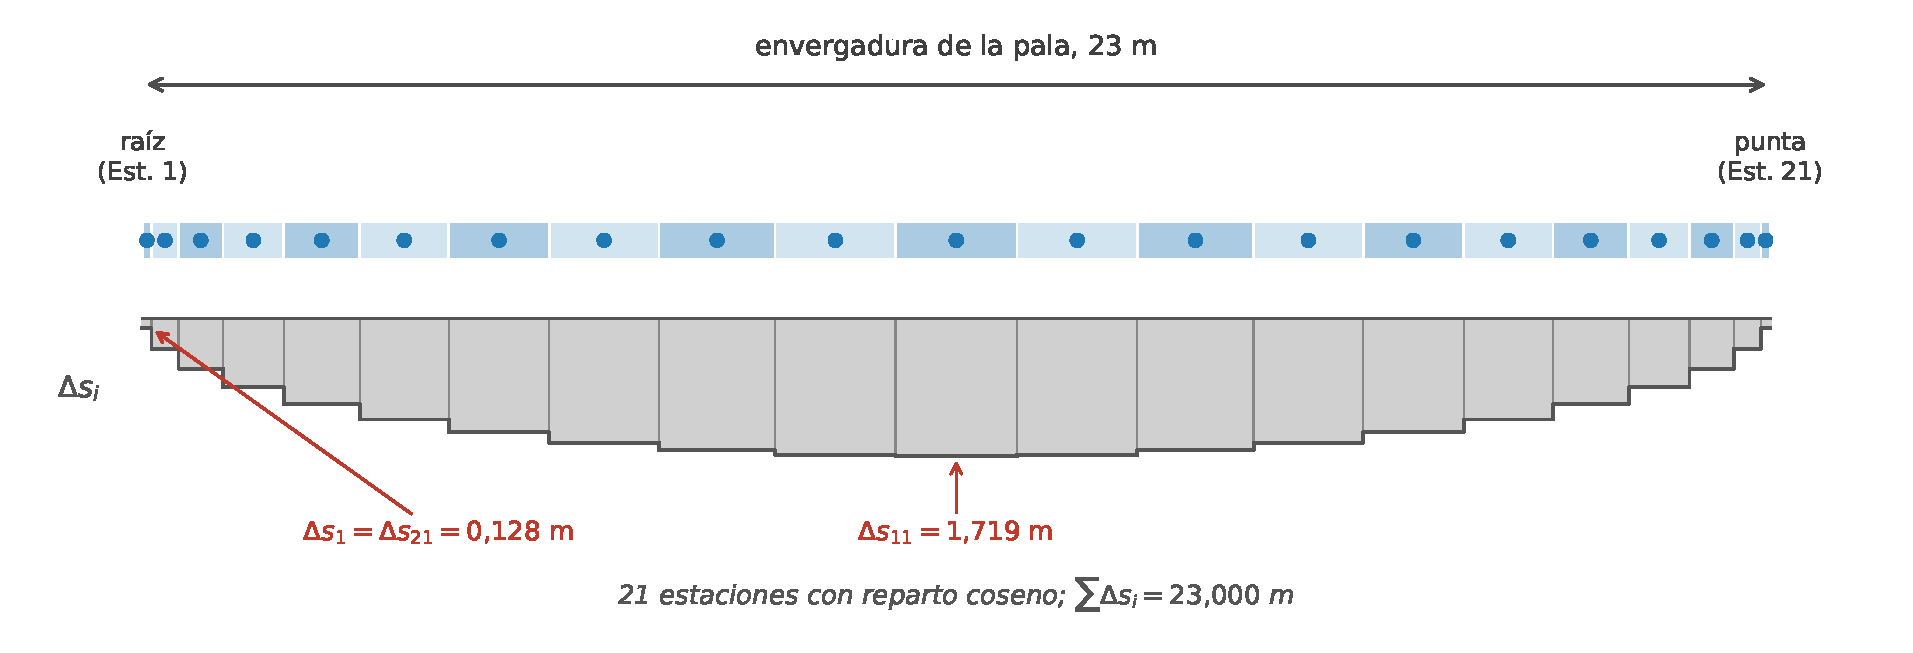
\includegraphics[width=0.95\textwidth]{Figuras/Figuras Metodología/estaciones_delta_s.pdf}
\caption[Tramo de pala que representa cada estación.]{Tramo de pala $\Delta s_i$ que representa cada una de las 24 estaciones.}
\label{fig:delta_s}
\end{figure}
 La raíz reúne las dos componentes en el módulo de la fuerza que actúa sobre cada estación, magnitud siempre positiva, de modo que la suma a lo largo de la envergadura no admite cancelaciones entre estaciones con carga de sentido opuesto y recoge la solicitación completa que soporta la pala.

\medskip
\noindent\textbf{Máximos por simulación y ajuste de Gumbel.}
Para cada velocidad de viento $V_j$ se dispone de $6$ simulaciones, una por semilla estocástica del campo de viento turbulento (Sección~\ref{sec:campo_turbulento}), de modo que las seis representan realizaciones independientes de un mismo proceso estocástico. De cada una se extrae el mayor valor que alcanza $F_{tot}(t)$ sobre el intervalo $t \geq 50$~s (Sección~\ref{sec:velocidades_simulacion}). Ese valor se denota $F_{max}$ y es la variable sobre la que opera todo el procedimiento que sigue: cada realización aporta una observación, de modo que a la velocidad $V_j$ se cuenta con seis. Extraer un único máximo por realización es coherente con la definición normativa de la carga característica, referida al mayor valor que se presenta en un intervalo de diez minutos (Sección 7.6.2 de la norma IEC 61400-1)~\parencite{IEC61400-1}.

Sobre esas seis observaciones se ajusta la distribución de Gumbel presentada en la Sección~\ref{sec:extrapolacion_teoria}, cuya función de distribución acumulada es la Ec.~\ref{eq:gumbel_anexof}, evaluada aquí en $F = F_{max}$. Sus dos parámetros, el de posición $\mu_j$ y el de escala $\beta_j$, se estiman por el método de los momentos, que iguala la media y la varianza de la distribución a las de la muestra. Para la distribución de Gumbel la media vale $\mu_j + \gamma_E \beta_j$ y la varianza $\pi^2 \beta_j^2 / 6$~\parencite{Gumbel1958}, de donde se despejan los estimadores de las Ecs.~\ref{eq:gumbel_beta} y~\ref{eq:gumbel_mu}:

\begin{equation}
    \beta_j = \frac{\sqrt{6}}{\pi}\,\sigma_{max,j}
    \label{eq:gumbel_beta}
\end{equation}

\begin{equation}
    \mu_j = \overline{F}_{max,j} - \gamma_E\,\beta_j
    \label{eq:gumbel_mu}
\end{equation}

donde $\overline{F}_{max,j}$ y $\sigma_{max,j}$ son la media y la desviación estándar de las seis observaciones de $F_{max}$ a la velocidad $V_j$, y $\gamma_E = 0{,}5772$ es la constante de Euler-Mascheroni~\parencite{Havil2003}. El subíndice $j$ recorre las doce velocidades simuladas, de manera que el ajuste entrega un par $(\mu_j, \beta_j)$ por cada una.

\medskip
\noindent\textbf{Probabilidad de excedencia condicionada a la velocidad.}
La Gumbel ajustada en el paso anterior permite calcular, para una velocidad fija $V_j$, la probabilidad de que $F_{max}$ supere un nivel de carga dado. En lo que sigue ese nivel se designa también $F_{max}$, por tratarse de la misma variable recién definida. La probabilidad condicional es el complemento de la función de distribución, según la Ec.~\ref{eq:pe_cond}:

\begin{equation}
    P_e(F_{max} \mid V_j) = 1 - \Phi(F_{max}; \mu_j, \beta_j)
    \label{eq:pe_cond}
\end{equation}

\medskip
\noindent\textbf{Integración de largo plazo con la distribución de Weibull.}
La probabilidad anterior está condicionada a una velocidad fija. Dado que cada velocidad $V_j$ ocurre con una frecuencia distinta a lo largo del año, se requiere la probabilidad de excedencia no condicionada. Para obtenerla, la norma prescribe integrar sobre la distribución de velocidades de viento en el emplazamiento (Ecuación F.2 del Anexo F de la norma IEC 61400-1)~\parencite{IEC61400-1}. Esa distribución es la densidad de Weibull de la Ec.~\ref{eq:weibull_pdf_general}, con los parámetros $k$ y $c$ ajustados a la altura del centro del rotor ($z = 21{,}3$~m) según el procedimiento de la Sección~\ref{sec:recurso_metodo}, cuyos valores se reportan en el Capítulo~4.

Numéricamente, la integral se discretiza en $N_V = 25$ intervalos de ancho $\Delta V = 1$~m/s, centrados en $V = 0{,}5; 1{,}5; \dots; 24{,}5$~m/s. Como solo se dispone de datos de Gumbel en las $12$ velocidades de simulación, los parámetros $\mu(V)$ y $\beta(V)$ se interpolan linealmente para los $25$ intervalos. La probabilidad de excedencia de largo plazo resulta según la Ec.~\ref{eq:pe_longterm}:

\begin{equation}
    P_e(F_{max}) = \sum_{m=1}^{N_V} \Bigl[1 - \exp\!\bigl(-e^{-(F_{max} - \mu(V_m))/\beta(V_m)}\bigr)\Bigr] \cdot f_W(V_m) \cdot \Delta V
    \label{eq:pe_longterm}
\end{equation}

En esta expresión, cada velocidad se pondera por su frecuencia de ocurrencia anual según la distribución de Weibull: las velocidades cercanas a $V_{ave}$ reciben mayor peso a pesar de producir fuerzas moderadas, mientras que las velocidades próximas a $V_{out}$ reciben menor peso aunque generan fuerzas mayores. La combinación de ambos efectos, frecuencia Weibull y magnitud Gumbel, determina la contribución relativa de cada velocidad al riesgo de excedencia a largo plazo.

\medskip
\noindent\textbf{Bisección para la carga característica a 50 años.}
La norma define la carga característica $F_k$ como aquella cuya probabilidad de ser superada en el período de retorno de diseño es exactamente $T_{obs} / T_{retorno}$, según la Ec.~\ref{eq:fk_criterion}:

\begin{equation}
    P_e(F_k) = \frac{T_{\text{obs}}}{T_{\text{retorno}}}
    \label{eq:fk_criterion}
\end{equation}

con $T_{obs} = 600$~s el período de observación de cada realización y $T_{retorno} = 50$ años el de diseño; el valor numérico de esta probabilidad objetivo se presenta en el Capítulo~4. La raíz $F_k$ se determina numéricamente por bisección sobre la Ec.~\ref{eq:pe_longterm}: se prueban valores de $F_{max}$, se evalúa $P_e(F_{max})$, y se ajusta el intervalo de búsqueda hasta alcanzar la probabilidad objetivo. La carga característica $F_k$ es el valor de $F_{max}$ que la satisface.

\medskip
\noindent\textbf{Carga de diseño.}
La carga característica $F_k$ es un valor estadístico; la carga de diseño $F_d$ incorpora además un margen para cubrir las incertidumbres del modelo de carga y de la extrapolación estadística. Se obtiene mayorando la carga característica por el factor parcial de carga, según la Ec.~\ref{eq:fd_anexof} de la Sección~\ref{sec:extrapolacion_teoria} (Ecuación 28, Sección 7.6.1.1 de la norma IEC 61400-1)~\parencite{IEC61400-1}, con $\gamma_f = 1{,}25$; ver su justificación en la Sección~\ref{sec:factores_seguridad}.

\medskip
\noindent\textbf{Perfil espacial de fuerzas de diseño.}
El Anexo F de la IEC 61400-1~\parencite{IEC61400-1} proporciona un único valor escalar $F_d$, que debe distribuirse a lo largo de la envergadura para cargar el modelo de elementos finitos. Esa distribución se resuelve en las mismas 24 estaciones con que se decidió instrumentar la pala (Sección~\ref{sec:discretizacion}), obteniéndose un vector de 24 fuerzas de diseño $(F_{d,x}[p], F_{d,y}[p])$, una por estación. Para preservar la correlación espacial entre estaciones, el perfil de carga se extrae del instante de máxima solicitación global en la realización que registró la mayor solicitación (Sección 7.5 de la norma IEC 61400-1)~\parencite{IEC61400-1}: se capturan las fuerzas compañeras $F_x[p], F_y[p]$ en ese $t_{max}$ y se escalan uniformemente por el factor $F_d / F_{tot}(t_{max})$. Este enfoque garantiza que la distribución espacial de fuerzas que ingresa al FEM sea la que entrega la simulación aerodinámica en ese único instante, con la correlación entre estaciones que ella misma produce, y no una combinación artificial de máximos independientes por estación que no ocurrieron simultáneamente; y que la magnitud global sea consistente con la carga de diseño a 50 años, ya que todas las estaciones provienen del mismo instante de la simulación. Las fuerzas se transfieren al modelo estructural conservando su signo, de modo que la dirección de aplicación reproduce la del instante gobernante. La Tabla~\ref{tab:anexo_fuerzas_dlc11} del \hyperref[anexo:fuerzas]{Anexo~A} presenta, para las 24 estaciones, tanto la fuerza $F_{sim,x}[p], F_{sim,y}[p]$ que entrega la simulación en el instante $t_{max}$ como la fuerza puntual de diseño $F_{d,x}[p], F_{d,y}[p]$ que resulta de escalarla y de aplicarla como carga remota en el modelo FEM; las direcciones $x$ e $y$ corresponden a los ejes locales de la Figura~\ref{fig:ejes_locales}.

\bigskip
\subsubsection{DLC 1.2 --- fatiga}
\label{sec:anexo_g}

Las mismas 72 series temporales empleadas para el DLC 1.1 se procesan conforme al Anexo G, informativo, de la IEC 61400-1~\parencite{IEC61400-1} para estimar el daño acumulado por fatiga durante la vida útil de diseño de $20$ años, valor que corresponde al mínimo exigido por la norma para las turbinas de clase I a III (Sección 6.2 de la norma IEC 61400-1)~\parencite{IEC61400-1}.

\medskip
\noindent\textbf{Variable de carga: momento flector en la sección crítica.}
En la configuración VAWT analizada, la pala se une al eje mediante dos brazos o \textit{struts} (Tabla~\ref{tab:geometria_turbina}), de modo que estructuralmente se comporta como una viga apoyada en esos dos puntos, con un tramo en voladizo en cada extremo. En cada instante de la simulación aerodinámica, las fuerzas distribuidas a lo largo de la envergadura flectan la pala y producen en cada sección transversal un momento flector, cuya magnitud depende de las fuerzas que actúan sobre el tramo que esa sección sostiene y de la distancia a la que lo hacen. El procedimiento de fatiga consiste, en términos simples, en calcular a partir de esas fuerzas el momento flector que soporta la sección más solicitada en cada instante, traducirlo a tensión mediante un factor de proporcionalidad calibrado con una única corrida del modelo de elementos finitos, y contar sobre la serie temporal de tensión así obtenida los ciclos que acumulan daño.

Se denomina sección crítica a la sección transversal de la pala en que la simulación FEM bajo carga estática (Sección~\ref{sec:fem}) registra la mayor tensión principal, y $z_{crit}$ a su coordenada sobre la envergadura, medida desde la base de la pala ($z = 0$) hasta esa sección. Su ubicación se desprende del análisis FEM y se reporta en el Capítulo~4.

El tramo que solicita a esa sección es el voladizo que ella sostiene, esto es, el conjunto de estaciones comprendidas entre el extremo libre de la pala y la sección crítica. Cuando la sección crítica corresponde a la conexión con el brazo inferior, ese tramo lo forman las estaciones situadas bajo ella, y las componentes del momento flector se obtienen según las Ecs.~\ref{eq:Mx_fatiga} y~\ref{eq:My_fatiga}:

\begin{align}
    M_x(t) &= \sum_{i:\, z_i < z_{crit}} F_{y,i}(t) \cdot (z_{crit} - z_i)
    \label{eq:Mx_fatiga} \\[4pt]
    M_y(t) &= \sum_{i:\, z_i < z_{crit}} F_{x,i}(t) \cdot (z_{crit} - z_i)
    \label{eq:My_fatiga} \\[4pt]
    M_{res}(t) &= \sqrt{M_x^2(t) + M_y^2(t)}
    \label{eq:Mres_fatiga}
\end{align}

donde el subíndice $i$ recorre las $24$ estaciones en que se discretizó la pala (Sección~\ref{sec:discretizacion}); $z_i$ es la coordenada de la estación $i$ sobre la envergadura (m) y $(z_{crit} - z_i)$, el brazo de palanca con que su carga actúa sobre la sección crítica; $F_{x,i}$ y $F_{y,i}$ son las fuerzas puntuales que aporta la estación $i$ en cada instante (N), obtenidas al multiplicar la fuerza por unidad de longitud que entrega la simulación por la longitud de pala $\Delta s_i$ que la estación representa, en las dos direcciones del sistema local de la Figura~\ref{fig:ejes_locales}. Las componentes $M_x$ y $M_y$ son los momentos flectores que actúan sobre la sección crítica en torno a cada uno de los dos ejes locales del perfil: $M_x$ flecta la pala en torno al eje $X_l$ y lo genera la componente de fuerza $F_y$, mientras que $M_y$ flecta en torno al eje $Y_l$ y lo genera $F_x$. El momento flector resultante $M_{res}$ es el módulo del vector que ambas componentes forman y constituye la variable de carga del análisis de fatiga. A diferencia de la fuerza total integrada $F_{tot}(t)$ empleada en el DLC 1.1, $M_{res}(t)$ se vincula directamente al mecanismo de falla por fatiga, ya que la tensión en la sección crítica es proporcional al momento resultante.

\medskip
\noindent\textbf{Conversión momento--tensión.}
Bajo la hipótesis de linealidad elástica del GFRP hasta rotura~\parencite{Huh2012,Moraras2023}, la tensión en el punto crítico admite descomponerse en dos contribuciones de naturaleza distinta. La aerodinámica fluctúa con el viento y es proporcional al momento flector resultante; la inercial, producida por la aceleración centrífuga y la gravedad, es constante mientras el rotor gira a su velocidad de consigna y no depende del momento aerodinámico. La historia de tensión en la sección crítica se construye en consecuencia según la Ec.~\ref{eq:sigma_from_M}:

\begin{equation}
    \sigma(t) = K_{aero} \cdot M_{res}(t) + \sigma_{in}
    \label{eq:sigma_from_M}
\end{equation}

donde $\sigma_{in}$ es la tensión principal máxima que el modelo FEM registra en la sección crítica bajo las cargas inerciales como única solicitación, y $K_{aero}$ el factor que traduce momento aerodinámico en tensión. Este último se obtiene de las mismas dos corridas del modelo FEM, según la Ec.~\ref{eq:keff}:

\begin{equation}
    K_{aero} = \frac{\sigma_{1,\max} - \sigma_{in}}{M_{res,d}}
    \label{eq:keff}
\end{equation}

donde $\sigma_{1,\max}$ es la tensión principal máxima bajo la carga de diseño completa del DLC 1.1, que incluye las cargas inerciales, y $M_{res,d}$ el momento flector resultante que producen las fuerzas aerodinámicas de diseño, evaluado mediante la Ec.~\ref{eq:Mres_fatiga}. Restar $\sigma_{in}$ del numerador aísla la fracción de tensión que efectivamente escala con el momento: calibrar el factor sobre la tensión total atribuiría al momento aerodinámico una contribución inercial que no depende de él, y sobreestimaría por ello la amplitud de todos los ciclos. Este enfoque es consistente con la formulación del Anexo G (Sección G.1 de la norma IEC 61400-1)~\parencite{IEC61400-1}, que permite asumir que la tensión local en el punto de falla es linealmente proporcional a la carga.

\medskip
\noindent\textbf{Conteo de ciclos Rainflow.}
Cada una de las 72 series temporales de tensión $\sigma(t)$, con una duración efectiva de $T_{sim} = 550$~s, se procesa mediante el algoritmo de conteo de ciclos Rainflow (Anexo G, Sección G.1 de la norma IEC 61400-1)~\parencite{IEC61400-1}, cuyo fundamento se expone en la Sección~\ref{sec:anexo_g_antecedentes}. La implementación empleada sigue la formulación de cuatro puntos normalizada en la práctica ASTM E1049-85~\parencite{ASTM_E1049}, correspondiente al método propuesto originalmente por \textcite{Matsuishi1968}. El algoritmo descompone la señal en ciclos individuales caracterizados por su amplitud $\sigma_a$ y su tensión media $\sigma_m$, preservando la secuencia de carga tal como ocurre en la simulación.

\medskip
\noindent\textbf{Corrección por tensión media.}
Cada ciclo se refiere a media nula mediante el diagrama de vida constante descrito en la Sección~\ref{sec:anexo_g_antecedentes}, con la tensión media $\sigma_m$ que entrega el propio conteo Rainflow y que incorpora, por construcción de la Ec.~\ref{eq:sigma_from_M}, la contribución inercial $\sigma_{in}$. Se adopta la formulación lineal de Goodman (Ec.~\ref{eq:goodman}) antes que la de Gerber porque \textcite{Huh2012}, la misma fuente de la que provienen la curva S-N y el exponente de fatiga empleados, contrasta ambas sobre este material y reporta que la de Goodman subestima la vida a fatiga del tejido bidireccional para tensiones medias superiores a $40$~MPa, esto es, resulta la conservadora de las dos en el rango que aquí interesa.

\medskip
\noindent\textbf{Curva S-N del material.}
La resistencia a fatiga del GFRP se modela mediante la ecuación de Basquin en su forma factorizada~\parencite{Basquin1910}. La norma prescribe que todos los factores parciales de seguridad se apliquen al rango de tensión cíclica (Sección 7.6.3 de la norma IEC 61400-1)~\parencite{IEC61400-1}, según la Ec.~\ref{eq:sigma_eq}:

\begin{equation}
    \sigma_{a,\text{eq}} = \gamma_f \cdot \gamma_m \cdot \gamma_n \cdot \sigma_{a,0}
    \label{eq:sigma_eq}
\end{equation}

donde $\sigma_{a,0}$ es la amplitud corregida por tensión media de la Ec.~\ref{eq:goodman}, y $\sigma_{a,\text{eq}}$ la amplitud de tensión equivalente de diseño, mayorada por los tres factores parciales de fatiga justificados en la Sección~\ref{sec:factores_seguridad}: $\gamma_f$ (carga), $\gamma_m$ (material) y $\gamma_n$ (consecuencia de falla).

La curva S-N de diseño, que relaciona la amplitud de tensión equivalente con el número de ciclos admisible, se expresa según la Ec.~\ref{eq:basquin_design}:

\begin{equation}
    \sigma_{a,\text{eq}} = \sigma_u \cdot (2N_f)^b
    \label{eq:basquin_design}
\end{equation}

Sustituyendo las Ecs.~\ref{eq:goodman} y~\ref{eq:sigma_eq} en la Ec.~\ref{eq:basquin_design} y despejando $N_f$ se obtiene la expresión utilizada en el cálculo de daño:

\begin{equation}
    N_{f} = \frac{1}{2}\left(\frac{\gamma_f \cdot \gamma_m \cdot \gamma_n}{\sigma_u} \cdot \frac{\sigma_{a}}{1 - \sigma_m / \sigma_u}\right)^{1/b}
    \label{eq:Nf_fatiga}
\end{equation}

donde $\sigma_u = 242{,}1$~MPa (resistencia última entregada por el fabricante de la pala, Tabla~\ref{tab:material_pala}), $b = -0{,}045$ (exponente de fatiga para tejido bidireccional $\pm 45^\circ$ fabricado por infusión al vacío~\parencite{Huh2012}) y $\gamma_f$, $\gamma_m$, $\gamma_n$ los factores parciales de fatiga justificados en la Sección~\ref{sec:factores_seguridad}.

\medskip
\noindent\textbf{Construcción del espectro colectivo anual.}
Cada simulación de $T_{sim} = 550$~s corresponde a una velocidad de viento fija $V_j$ y produce, mediante Rainflow, un conjunto de ciclos de fatiga $(\sigma_a, \sigma_m)$. Estos ciclos representan la operación continua del aerogenerador durante $550$~s a dicha velocidad. Para construir el espectro representativo de un año completo, los ciclos de cada velocidad se expanden proporcionalmente a la fracción de tiempo que el viento permanece en ese intervalo en el emplazamiento.

La fracción de tiempo anual asociada a la velocidad $V_j$ se obtiene de la distribución de Weibull que caracteriza el sitio (Ec.~\ref{eq:weibull_pdf_general}), según la Ec.~\ref{eq:tiempo_anual}:

\begin{equation}
    t_j = f_W(V_j) \cdot \Delta V \cdot 365{,}25 \cdot 24 \cdot 3600 \quad [\text{s/año}]
    \label{eq:tiempo_anual}
\end{equation}

donde $f_W(V_j)$ es la densidad de probabilidad Weibull evaluada en $V_j$, $\Delta V = 2$~m/s es el ancho del intervalo de velocidad, y $365{,}25 \cdot 24 \cdot 3600$ es la duración de un año calendario en segundos, considerando el promedio de $365{,}25$ días que incorpora los años bisiestos; no es un valor prescrito por la norma, sino la conversión que lleva la densidad de probabilidad a una tasa temporal. La Tabla~\ref{tab:weibull_fatiga} en el Capítulo~4 presenta, para las doce velocidades $V_j$ del rango operacional, los valores de $f_W(V_j)$, $t_j$ y el factor de escalamiento temporal $t_j / T_{sim}$.

El número de ciclos anuales atribuibles a la velocidad $V_j$ se calcula escalando los ciclos simulados (Ecuación G.7 del Anexo G de la norma IEC 61400-1)~\parencite{IEC61400-1}, según la Ec.~\ref{eq:espectro_anual}:

\begin{equation}
    n_{j}^{\text{anual}} = \bar{n}_{j}^{\text{sim}} \cdot \frac{t_j}{T_{sim}}
    \label{eq:espectro_anual}
\end{equation}

donde $\bar{n}_{j}^{\text{sim}}$ es el número promedio de ciclos de las $6$ semillas a la velocidad $V_j$, es decir, de las seis series generadas con una semilla estocástica distinta, el entero que inicializa el generador de números aleatorios del campo de turbulencia y que hace que cada serie sea una realización independiente del mismo proceso estocástico (Sección~\ref{sec:campo_turbulento}). Las $72$ series simuladas ($12$ velocidades $\times$ $6$ semillas) se agrupan por velocidad de viento y los ciclos de las $6$ semillas se promedian antes del escalamiento temporal para reducir la variabilidad estocástica. El espectro colectivo anual se construye sumando las contribuciones de las $12$ velocidades que cubren el rango operacional; es este conjunto combinado de ciclos, indexado por $i$, el que recorre la suma de la Ec.~\ref{eq:palmgren_miner}.

\medskip
\noindent\textbf{Daño acumulado.}
El daño total por fatiga se evalúa mediante la regla de Palmgren-Miner~\parencite{Miner1945}, que asume acumulación lineal e independiente de cada ciclo, criterio que la norma adopta en su Anexo G, Sección G.1~\parencite{IEC61400-1}, según la Ec.~\ref{eq:palmgren_miner}:

\begin{equation}
    D_{\text{año}} = \sum_{i} \frac{n_i^{\text{anual}}}{N_{f,i}}
    \label{eq:palmgren_miner}
\end{equation}

donde $D_{\text{año}}$ es el daño acumulado por fatiga durante un año de operación, $n_i^{\text{anual}}$ es el número de ciclos anuales correspondientes a la amplitud de tensión $\sigma_{a,i}$, y $N_{f,i}$ es el número de ciclos admisible para dicha amplitud, determinado mediante la Ec.~\ref{eq:Nf_fatiga}. El daño total para la vida útil de diseño de $20$ años se obtiene por acumulación lineal, según la Ec.~\ref{eq:D20}:

\begin{equation}
    D_{20} = 20 \cdot D_{\text{año}}
    \label{eq:D20}
\end{equation}

La verificación del estado límite de fatiga exige que el daño acumulado no supere la unidad, según la Ec.~\ref{eq:fatiga_criterio} (Sección 7.6.3 de la norma IEC 61400-1)~\parencite{IEC61400-1}:

\begin{equation}
    D_{20} \leq 1{,}0
    \label{eq:fatiga_criterio}
\end{equation}

\bigskip
\subsubsection{DLC 1.3 --- estado límite último}
\label{sec:anexo_dlc13}

Para el DLC 1.3, la norma prescribe un método alternativo al Anexo F. Las cargas características se determinan como la media de los máximos de las realizaciones estocásticas, sin extrapolación temporal a 50 años (Sección 7.6.2 de IEC 61400-1~\parencite{IEC61400-1}).

\medskip
\noindent\textbf{Extracción de máximos.}
La fuerza total integrada $F_{tot}(t)$ es la misma señal escalar definida en la Ec.~\ref{eq:F_tot} para el DLC 1.1: la integración es espacial, sobre las 24 estaciones de la pala en cada instante, y por sí sola no incluye ninguna búsqueda de máximos. Se calcula de igual forma para cada una de las simulaciones del DLC 1.3 y, a partir de ella, para cada velocidad $V_j$ ($j = 1,\dots,5$, correspondientes a $V = 16$, $18$, $20$, $22$ y $24$~m/s) se extraen los $6$ máximos $F_{tot,\max}(V_j, s)$ con $s = 1,\dots,6$, sobre el intervalo $t \geq 50$~s.

\medskip
\noindent\textbf{Carga característica por velocidad.}
A diferencia del DLC 1.1, donde el Anexo F ajusta una distribución de extremos y extrapola sobre todo el rango operacional, la Sección 7.6.2 de la norma IEC 61400-1~\parencite{IEC61400-1} define aquí la carga característica sin extrapolación temporal: para una velocidad de viento dada, es la media de los máximos de las realizaciones estocásticas disponibles a esa velocidad. Para cada una de las cinco velocidades $V_j$ ensayadas en el DLC 1.3, la carga característica $F_k(V_j)$ se calcula, en consecuencia, como el promedio aritmético de los $6$ máximos $F_{tot,\max}(V_j, s)$ obtenidos en el paso anterior, uno por semilla, según la Ec.~\ref{eq:dlc13_Fk_local}:

\begin{equation}
    F_k(V_j) = \frac{1}{6}\sum_{s=1}^{6} F_{tot,\max}(V_j, s)
    \label{eq:dlc13_Fk_local}
\end{equation}

donde $F_{tot,\max}(V_j, s)$ es el máximo de $F_{tot}(t)$ de la simulación de semilla $s$ a la velocidad $V_j$, extraído en el paso anterior. Este cálculo se repite de forma independiente para cada una de las cinco velocidades ensayadas, lo que entrega un conjunto de cinco cargas características $F_k(V_j)$, una por velocidad.

La carga característica global del DLC 1.3, $F_k$, es la mayor de esas cinco cargas, y la velocidad que la produce se denomina velocidad gobernante, $V_{gob}$, por ser la que domina el caso de carga. Esta carga se amplifica por el factor $\gamma_f = 1{,}35$; ver su justificación en la Sección~\ref{sec:factores_seguridad}. El perfil espacial de diseño se construye como la media por estación de los perfiles compañeros de las $6$ semillas a la velocidad gobernante, amplificada por el mismo factor, lo que preserva la coherencia entre la carga global y su distribución a lo largo de la envergadura.

\section{Etapa 3: análisis estructural}

\subsection{Material de la pala}
\label{sec:material_pala}

La pala está construida en material compuesto de polímero reforzado con fibra de vidrio (GFRP), fabricado mediante infusión al vacío. El perímetro $P$ de la sección transversal NACA 0018 se obtiene al integrar numéricamente el contorno normalizado del perfil de la Figura~\ref{fig:naca0018}, lo que entrega la relación de la Ec.~\ref{eq:perimetro_naca}:

\begin{equation}
    P \approx 2{,}08 \, c
    \label{eq:perimetro_naca}
\end{equation}

donde $c$ es la cuerda del perfil (Tabla~\ref{tab:geometria_turbina}). Con base en la masa total de la pala equivalente a $760$ kg, proporcionada por el fabricante de la turbina, la densidad del material ($\rho = 1\,800$~kg/m$^3$, Tabla~\ref{tab:material_pala}) y el perímetro de la Ec.~\ref{eq:perimetro_naca}, se estima un espesor de pared equivalente de $8$ mm para el modelo estructural. El modelo incorpora además un larguero interior que recorre la envergadura completa en la zona de espesor máximo del perfil. Ante la ausencia de una definición del laminado y de la estructura interna, el espesor del larguero se fija igual al del manto ($8$~mm); la sensibilidad de los resultados a este supuesto se evalúa en el análisis de estabilidad (Sección~\ref{sec:pandeo_met}). La incorporación del larguero añade del orden de un $8\%$ de masa respecto del valor nominal de la pala, desviación que se acepta por tratarse de un elemento estructuralmente necesario, como se demuestra en el Capítulo~4. Cabe señalar que la omisión del larguero interior es una alternativa que el fabricante evalúa para facilitar la fabricación de la pala. Las propiedades mecánicas del material se resumen en la Tabla~\ref{tab:material_pala}.

\begin{table}[H]
    \centering
    \caption{Propiedades del material compuesto GFRP de la pala y su procedencia.}
    \label{tab:material_pala}
    \begin{tabular}{lccl}
        \hline
        \textbf{Propiedad} & \textbf{Símbolo} & \textbf{Valor} & \textbf{Procedencia}\\
        \hline
        Densidad & $\rho$ & $1\,800$~kg/m$^3$ & Fabricante de la pala\\
        Módulo elástico & $E$ & $38{,}208$ GPa & Fabricante de la pala\\
        Coeficiente de Poisson & $\nu$ & $0{,}30$ & Fabricante de la pala\\
        Resistencia última & $\sigma_u$ & $242{,}1$ MPa & Fabricante de la pala\\
        Espesor de pared equivalente & — & $8$ mm & Estimado de la masa de la pala\\
        Exponente de fatiga & $b$ & $-0{,}045$ & Literatura~\parencite{Huh2012}\\
        \hline
        \multicolumn{4}{l}{\footnotesize El tipo de material (GFRP fabricado por infusión al vacío) es dato del fabricante de la pala.}
    \end{tabular}
\end{table}

El GFRP presenta un comportamiento elástico lineal hasta la rotura frágil~\parencite{Huh2012,Moraras2023}. La Figura~\ref{fig:curva_esfuerzo_deformacion} presenta la curva esfuerzo-deformación construida a partir de las propiedades entregadas por el fabricante de la pala (Tabla~\ref{tab:material_pala}), donde la pendiente de la recta corresponde al módulo elástico $E = 38{,}208$~GPa y el punto de rotura se alcanza a una deformación $\varepsilon_u = 0{,}63\%$ bajo un esfuerzo $\sigma_u = 242{,}1$~MPa.

\begin{figure}[H]
    \centering
    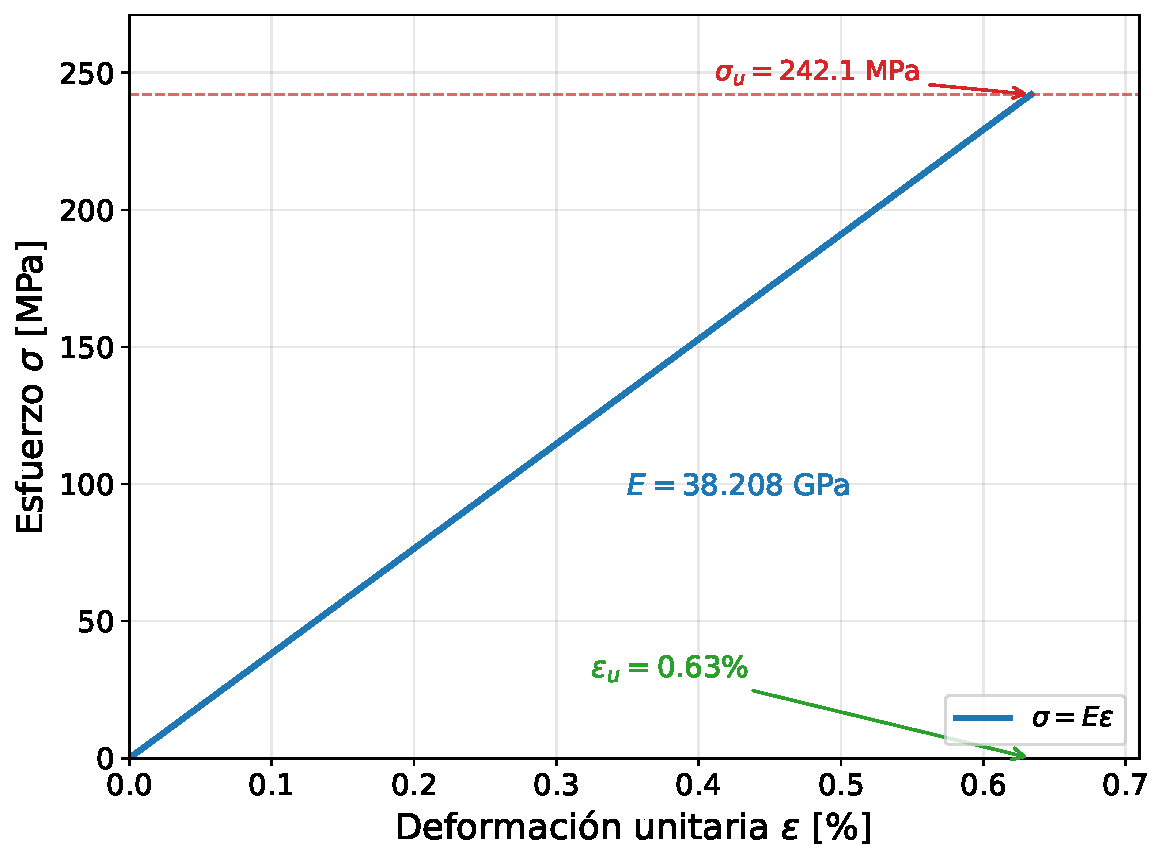
\includegraphics[width=0.65\textwidth]{Figuras/Figuras Metodología/curva_esfuerzo_deformacion.pdf}
    \caption{Curva esfuerzo-deformación del GFRP $\pm 45^\circ$ de la pala, construida a partir de las propiedades entregadas por el fabricante.}
    \label{fig:curva_esfuerzo_deformacion}
\end{figure}

Las propiedades disponibles del laminado son las de la Tabla~\ref{tab:material_pala}: un módulo elástico, un coeficiente de Poisson y una resistencia única, esto es, un conjunto isótropo equivalente. Sobre esa base el material se modela como isótropo lineal. Dos condiciones del análisis hacen consistente esa representación. La primera es que la pala está construida íntegramente con el mismo laminado, de modo que el modelo no debe reproducir desajustes de rigidez entre la piel y el larguero. La segunda es que la verificación de resistencia última emplea el criterio de tensión principal máxima, que compara una tensión escalar con una resistencia única y no requiere descomponer el estado tensional en las direcciones del refuerzo. El alcance de la hipótesis se retoma en las conclusiones.

\subsection{Análisis por modelado de elementos finitos de la pala}
\label{sec:fem}

El análisis estructural de la pala se realiza en el software Ansys. En correlación con los objetivos propuestos, se modela únicamente una pala, excluyendo los struts, la torre y el sistema de flotación del dominio de cálculo. La exclusión del sistema de flotación responde, además, a la falta de datos para modelarlo: el fabricante no entrega su geometría ni sus propiedades, información que resguarda por confidencialidad comercial. La discretización emplea las mismas 24 estaciones adoptadas para instrumentar la pala en QBlade (Sección~\ref{sec:discretizacion}), lo que permite trasladar directamente las cargas sin requerir interpolación entre dominios.

\subsubsection{Condiciones de borde}
\label{sec:condiciones_borde}

La pala se sostiene en los dos puntos en que se conecta a los brazos, situados a $z = 5{,}0$ y $z = 17{,}0$~m sobre la base (Tabla~\ref{tab:geometria_turbina}), que constituyen por tanto sus únicos apoyos. Ambos se representan como empotramientos, esto es, restringiendo los seis grados de libertad, criterio coherente con la rigidez del conjunto brazo-eje frente a la de la pala y con la exclusión de los brazos del dominio de cálculo. La restricción no se impone sobre una arista ni sobre un nodo, sino sobre una superficie de $500 \times 600$~mm en cada conexión, de modo que la reacción se reparte sobre un área finita y no genera la singularidad de tensión que produciría un apoyo puntual. Bajo estas condiciones la pala se comporta como una viga con dos apoyos y un voladizo en cada extremo, configuración que determina las zonas críticas del análisis.

La zona de conexión incorpora además un vendaje de refuerzo de $20$~mm de espesor y $1$~m de longitud, dispuesto concéntricamente alrededor del perímetro de la sección, que reproduce el engrosamiento local del laminado con que se resuelve la introducción de carga en una unión de este tipo.

\subsubsection{Cargas aplicadas}

Las fuerzas aerodinámicas se aplican según el procesamiento de datos específico de cada caso. Además de ellas, se aplican las cargas másicas de origen inercial, que por su naturaleza determinística no requieren extrapolación estadística. Estas no se introducen como fuerzas nodales, sino como aceleraciones globales impuestas sobre la totalidad del modelo: el solucionador las convierte en fuerzas de volumen elemento a elemento, multiplicando la masa de cada elemento por la aceleración prescrita, de modo que la distribución espacial de la carga inercial queda determinada por la distribución de masa del propio modelo. Las aceleraciones que definen estas cargas son:

\begin{itemize}
    \item \textbf{Aceleración de gravedad:} uniforme, dirigida verticalmente hacia abajo y de magnitud $g = 9{,}81$~m/s$^2$.
    \item \textbf{Aceleración centrífuga:} dirigida radialmente hacia afuera, producida por la rotación del rotor y evaluada en la velocidad máxima de rotación $\Omega$ mediante la Ec.~\ref{eq:centrifugal_limit} (Sección~\ref{sec:vtip}). Por tratarse de un H-rotor de palas rectas paralelas al eje, el radio $R$ es constante a lo largo de la envergadura, de modo que la aceleración resulta uniforme en toda la pala y admite imponerse como un único campo global. El valor que corresponde a la consigna de rotación adoptada se presenta en el Capítulo~4.
\end{itemize}

\subsubsection{Discretización de la malla}

La pala se discretiza mediante elementos sólidos tridimensionales de tipo hexaédrico dominante, discretización que \textcite{HAND2021} emplean y validan para el análisis estructural por elementos finitos de palas de \gls{vawt}. El calificativo dominante indica que en las regiones donde la geometría no admite el barrido hexaédrico, como las transiciones de espesor y los encuentros con el larguero, el mallador recurre localmente a elementos de transición.

Para garantizar la independencia de los resultados respecto del tamaño de malla, se realiza un análisis de convergencia variando progresivamente la densidad de elementos hasta que la variación en la tensión principal máxima entre mallas sucesivas sea inferior al $5\%$, umbral establecido en la literatura para análisis de elementos finitos~\parencite{Qin2026} y empleado en estudios de palas eólicas~\parencite{Hameed2015,Boudounit2020}. Este procedimiento elimina la influencia de concentradores de esfuerzos propios de la discretización.

A partir del análisis se obtienen la tensión principal máxima ($\sigma_1$), las deformaciones unitarias y los desplazamientos nodales. La verificación de resistencia última se realiza mediante el criterio de máxima tensión principal, apropiado para materiales compuestos de matriz polimérica con comportamiento frágil~\parencite{Moraras2023}. Al representar el laminado como un sólido homogéneo, la verificación aborda la rotura gobernada por las fibras y no resuelve los mecanismos interlaminares descritos en la Sección~\ref{sec:comportamiento_laminado}. El criterio se aplica comparando $\sigma_{1,\max}$ con la resistencia última factoreada del material, cuyas propiedades mecánicas proporciona el fabricante de la turbina.

\subsubsection{Verificación de estabilidad (pandeo)}
\label{sec:pandeo_met}

La verificación de estabilidad exigida por la Sección 7.6.4 de la norma IEC 61400-1~\parencite{IEC61400-1} se realiza mediante un análisis de pandeo lineal por autovalores (\textit{Eigenvalue Buckling}) en Ansys, según el planteamiento de la Ec.~\ref{eq:pandeo_autovalores} de la Sección~\ref{sec:pandeo_teoria}, acoplado a las soluciones estáticas de ambos casos de carga última (DLC 1.1 y 1.3), de las cuales hereda la malla, las cargas y las condiciones de borde. La simulación entrega el multiplicador de carga (\textit{load multiplier}, $LM$) de cada modo, es decir, el factor por el que deberían amplificarse las cargas aplicadas para alcanzar la inestabilidad elástica, y se extraen los tres primeros modos.

Dado que las cargas aplicadas ya incorporan el factor parcial $\gamma_f$, la condición de verificación se plantea del lado de la resistencia con los mismos factores parciales de la verificación de resistencia última, según la Ec.~\ref{eq:criterio_pandeo}:

\begin{equation}
    LM \geq \gamma_m \cdot \gamma_n = 1{,}30
    \label{eq:criterio_pandeo}
\end{equation}

donde $\gamma_m = 1{,}30$ y $\gamma_n = 1{,}00$ son los factores parciales de resistencia última de la Tabla~\ref{tab:factores_seguridad}. El criterio exige, por tanto, que el modo crítico no se alcance antes de amplificar las cargas de diseño en un $30\%$.

Cabe señalar que el método lineal por autovalores no incorpora imperfecciones geométricas ni efectos no lineales, a los que los cascarones de pared delgada son sensibles, por lo que sus resultados constituyen una cota superior de la carga crítica real (Sección~\ref{sec:pandeo_teoria}).

Junto al caso base, con piel y larguero de $8$~mm, se resuelven dos variantes que acotan el origen del margen obtenido, ambas sobre el caso de carga gobernante y con idénticas condiciones de borde. La primera suprime el larguero interior, con lo que se evalúa la alternativa de fabricación que plantea el fabricante (Sección~\ref{sec:material_pala}). La segunda aumenta el espesor del larguero a $12$~mm, manteniendo la piel en $8$~mm, con lo que se comprueba la sensibilidad del resultado al supuesto adoptado para ese espesor ante la falta de una definición del laminado. Ambas variantes permiten discriminar si la capacidad del conjunto la gobierna el larguero o los paneles de piel, distinción que determina hacia dónde debe dirigirse un eventual refuerzo.

